\documentclass[twoside,11pt]{article}
\usepackage[preprint]{jmlr2e}
\usepackage{booktabs}
\usepackage{tabularx}
\usepackage{array}
\usepackage{amsmath}
\usepackage{graphicx}
\usepackage{url}

\jmlrheading{}{2026}{}{}{}{}{Kassim et al.}
\ShortHeadings{kodama-cpp supplement}{Kassim et al.}
\firstpageno{1}

\begin{document}
\title{Technical Supplement: kodama-cpp}
\author{%
\name Moussa Kassim$^{1,2,*}$ \email moussa.kassim@icgeb.org \\
\name Martin Ocharo$^{1,2,*}$ \email martin.ocharo@icgeb.org \\
\name Dalia Ahmed$^{1}$ \email dalia.ahmed@icgeb.org \\
\name Dupe Ojo$^{1}$ \email dupe.ojo@icgeb.org \\
\name Alessia Vignoli$^{3,4}$ \email vignoli@cerm.unifi.it \\
\name Leonardo Tenori$^{3,4,\dagger}$ \email tenori@cerm.unifi.it \\
\name Dinesh Gupta$^{20}$ \\
\name Silvano Piazza$^{21,22}$ \\
\name Stefano Cacciatore$^{1,2,\dagger}$ \email stefano.cacciatore@icgeb.org \\
\addr $^{1}$ Bioinformatics Unit, International Centre for Genetic Engineering and Biotechnology (ICGEB), Cape Town 7925, South Africa \\
\addr $^{2}$ Department of Integrative Biomedical Sciences, \\ \addr Institute of Infectious Disease \& Molecular Medicine (IDM), \\ \addr University of Cape Town, Cape Town 7925, South Africa \\
\addr $^{3}$ Department of Chemistry ``Ugo Schiff'', University of Florence, Sesto Fiorentino, Italy \\
\addr $^{4}$ Magnetic Resonance Center (CERM), University of Florence, Sesto Fiorentino, Italy \\
\addr $^{20}$ Translational Bioinformatics Group, International Centre for Genetic Engineering and Biotechnology (ICGEB), New Delhi, India \\
\addr $^{21}$ Computational Biology Group, International Centre for Genetic Engineering and Biotechnology (ICGEB), Trieste, Italy \\
\addr $^{22}$ Bioinformatics Facility, Department of Cellular, Computational and Integrative Biology -- CIBIO, University of Trento, Trento, Italy \\
\addr $^{*}$ Moussa Kassim and Martin Ocharo contributed equally. \\
\addr $^{\dagger}$ Leonardo Tenori and Stefano Cacciatore are co-corresponding authors. \\
}
\maketitle
\begin{abstract}
KODAMA searches for latent structure by maximizing the cross-validated predictability of an evolving label vector. We present kodama-cpp and make five contributions. First, KODAMA is implemented as a standalone C++17 library with a typed, wrapper-independent API, allowing thin R and Python interfaces to share one numerical implementation. Second, native multicore CPU, NVIDIA CUDA, and Apple Metal backends implement float32 nearest-neighbor search, k-means, PCA, graph operations, and reusable workspaces without silent CPU fallback. Third, kodama-cpp introduces label-aware SIMPLS followed by LDA in the requested-component latent space as a new KODAMA evaluator, distinct from the historical PLS-DA decoder. Fourth, the current search uses a common prediction-guided proposal and evaluation scaffold, while PLS-LDA adds a disclosed transition-coarsening move and fragmentation term to its state score. Proposal size decreases smoothly, an error-scaled temperature permits early exploration, and each cycle performs exactly one new cross-validation pass. Fifth, the landmark-projection strategy is formalized for general matrix input through exact-quota stratified sampling, optimization on landmarks, and supervised projection to the remaining samples. These policies retain cross-validated predictability as the internal signal but need not reproduce historical stochastic trajectories. We validate backend identity, numerical behavior, runtime, memory, landmark-selection contracts, and external-label diagnostics separately so that systems acceleration is not conflated with the optimization objective. In an explicitly exploratory 10-dataset matched analysis, PLS-LDA KODAMA followed by UMAP improved truth-label silhouette on six datasets (median change +0.025, bootstrap 95\% interval [-0.067, +0.084]); KNN and openTSNE were less favorable, precluding a universal claim.
\end{abstract}
\begin{keywords}
KODAMA, unsupervised learning, cross-validation, heterogeneous computing, CUDA, Metal, C++ library, nearest neighbors, PLS-LDA
\end{keywords}

\section{Scope}
This supplement contains the information needed to reproduce the mathematical and software claims in the four-page JMLR MLOSS description. It is organized by contract rather than development date: exact KODAMA mathematics, pseudocode, architecture and backend invariants, benchmark protocol, decisive current evidence, limitations, and provenance. Historical optimization attempts and rejected prototypes are retained as dated repository reports and are not reproduced here.

The original KODAMA paper introduced this idea as knowledge discovery by accuracy maximization, and the subsequent R package made it available as an unsupervised and semi-supervised feature-extraction tool for noisy high-dimensional data. The Bioinformatics package paper describes the algorithm as repeated random label initialization, iterative maximization of cross-validated accuracy by label swapping, and construction of a dissimilarity matrix from the resulting label vectors. The R documentation exposes the same logic through M independent iterative processes, Tcycle optimization steps, KNN or PLS-DA classifiers, and separate KODAMA.matrix and KODAMA.visualization functions.

The repeated classifier fits inside KODAMA create a systems problem that is not resolved by translating individual R expressions into C++. Neighbor indices, fold matrices, class encodings, latent projections, and evolving labels must be reused across many cross-validation calls without changing the accepted label trajectory. A useful accelerator implementation must therefore preserve the mathematical state machine while changing where that state lives and how it moves.

kodama-cpp addresses this problem with a standalone C++17 core and explicit CPU, CUDA, and Apple Metal backends. It currently supports two classifier families in the KODAMA optimization layer: KNN for local neighborhood consistency and PLS-LDA for low-rank linear discrimination. R and Python wrappers call the same typed API, so fold construction, proposals, acceptance decisions, and result metadata are not reimplemented by each language interface. Their public functions, defaults, accepted choices, one-based best-run convention, and result fields are matched; Python only transliterates dotted R argument names to snake\_case.

The manuscript is organized around five novelties. The first is software ownership: KODAMA becomes a standalone C++ library from which R and Python wrappers can be built without reimplementing folds, proposals, classifiers, or graph construction. The second is heterogeneous execution through native CUDA and Apple Metal backends under the same float32 result contract. The third is a label-aware SIMPLS evaluator followed by LDA in the requested-component latent space, a new KODAMA classifier route rather than a reimplementation of the historical PLS-DA decoder. The fourth is a guided label-evolution strategy that uses out-of-fold predictions, class-transition evidence, adaptive proposal sizes, degeneracy guards, and error-scaled cooling while preserving one new CV evaluation per cycle. The fifth is a general landmark-projection procedure that makes the expensive optimization depend on a representative subset and then projects each optimized solution to all samples.

We deliberately frame this contribution as a software-methods paper, not as a claim that KODAMA replaces clustering, semi-supervised learning, or manifold learning. Cross-validated accuracy is the internal optimization criterion used to construct candidate label vectors. External labels, when available, are used only for diagnostics such as adjusted Rand index, silhouette, local purity, and runtime-quality tradeoffs.

\begin{table}[h]
\caption{Main contributions of kodama-cpp.}
\small
\begin{tabularx}{\linewidth}{p{0.24\linewidth}X}
\toprule
Contribution & Role in kodama-cpp \\
\midrule
Standalone C++ core & Moves folds, classifiers, label evolution, projection, and graph construction into one C++17 library so thin R and Python wrappers share the same typed implementation. \\
CUDA and Metal backends & Provides native float32 KNN, k-means, SIMPLS-LDA, PCA, and reusable accelerator state with strict backend identity and no silent CPU fallback. \\
Guided CV maximization & Uses a common prediction-guided proposal/evaluation scaffold; PLS-LDA additionally applies transition coarsening and a fragmentation-aware state-score term. \\
Landmark projection & Uses exact-quota stratified sampling, optimization on a representative subset, supervised projection, and ensemble graph correction. \\
\bottomrule
\end{tabularx}
\end{table}

\section{KODAMA objective}
Let X in R\textasciicircum{}(n x p) denote the input matrix, c in \{1,...,K\}\textasciicircum{}n a candidate label vector, F a classifier family, and Pi a fold assignment. For each validation sample i, the classifier is trained on samples not in Pi(i) and predicts c\_i from x\_i. The empirical objective is the held-out accuracy A(c; X, F, Pi). KODAMA searches for a labeling c* that maximizes this quantity, turning unsupervised structure discovery into a self-guided supervised prediction problem.

One KODAMA run starts from an initial partition. In the historical R interface, this can be one label per sample or a clustering-derived vector W; a fraction of samples can be selected for each run, with 75\% as the documented default. The current C++ interface keeps the same idea but exposes starting labels, splitting, landmarks, and fixed or constrained groups as typed inputs. During each cycle, misclassified samples or constrained groups generate candidate label moves. A move is accepted if it improves the objective, or under a temperature rule that allows exploration early in the run. Landmark projection is treated as a general matrix algorithm: label optimization is performed on selected landmarks and the chosen classifier restores a complete label vector before ensemble construction.

The M runs are independent. This independence is important both statistically, because it averages over random initialization and proposal order, and computationally, because backend schedulers can process runs without changing the objective. The final KODAMA representation is obtained from the ensemble of optimized label vectors: pairs of samples that repeatedly receive compatible labels are pulled closer in the derived graph or dissimilarity, while unstable pairs are weakened.

\section{Mathematical specification}
\subsection{Cross-validated predictability}
Let $X\in\mathbb{R}^{n\times p}$, candidate labels $y\in\{1,\ldots,K\}^{n}$, classifier family $F$, and fold assignment $\Pi$. Training excludes the fold containing validation sample $i$. The raw held-out accuracy is
\begin{equation}
A(y;X,F,\Pi)=\frac{1}{n}\sum_{i=1}^{n}
\mathbf{1}\!\left[y_i=\widehat y_i^{(-\Pi(i))}\right].
\end{equation}
Folds remain fixed within one independent run. A supplied constraint vector assigns an entire group to one fold and makes that group the atomic relabeling unit. A supplied fixed mask prevents relabeling without removing the sample from CV.

\subsection{Landmark-projection strategy}
Landmark projection reduces the cost of repeated accuracy maximization by optimizing labels only on a selected subset, fitting a supervised model to each optimized landmark vector, and predicting labels for the remaining samples before constructing the ensemble dissimilarity. kodama-cpp implements this as a general algorithmic component for matrix inputs that does not depend on a wrapper language.

The current selector replaces k-means with one center per requested landmark by a coarse partition followed by exact population-proportional allocation. For effective landmark count L and coarse stratum c containing n\_c of n samples, q\_c = L n\_c / n is the expected allocation. The algorithm samples floor(q\_c) rows without replacement, then assigns the remaining slots by randomized systematic rounding of the fractional quotas. It therefore returns exactly L distinct landmarks and satisfies E[L\_c] = L n\_c / n without requiring L k-means centers.

Sampling strata and labels being optimized are intentionally different objects. After landmarks are selected, a separate expression-space partition initializes the candidate labels. KODAMA evolves those labels for Tcycle steps, stores the selected vector from each of M independent runs, and projects it to non-landmarks with the selected KNN or PLS-LDA classifier. The final graph is then corrected from agreement across complete projected vectors, so non-landmarks contribute to the returned representation even though the iterative CV search is performed on the landmark subset.

\begin{table}[h]
\caption{Validation of the landmark-projection implementation.}
\small
\begin{tabularx}{\linewidth}{p{0.22\linewidth}X}
\toprule
Validation dimension & Current manuscript evidence \\
\midrule
Selection contract & Unit tests require the exact effective landmark count, distinct sampled rows, fixed-seed repeatability, and valid represented/occupied-stratum diagnostics. \\
Backend contract & CPU and CUDA matrix runs expose matching landmark counts and diagnostics; selection remains host-orchestrated and independent of classifier backend. \\
Scalability isolation & On flow18, selecting 750,016 landmarks from 300 coarse strata required 0.321 seconds. Recall-tuned resident CUDA IVF-Flat subsequently reduced the 100-neighbor graph from 296.482 to 25.938 seconds. \\
Quality evaluation & Landmark tests report downstream CV accuracy, ensemble stability, and external diagnostics separately from selection time so representativeness is not inferred from speed alone. \\
\bottomrule
\end{tabularx}
\end{table}

\subsection{Label-vector search mechanics}
The object optimized by KODAMA is the label vector itself. At any time the algorithm holds a candidate vector y on the landmark samples. A classifier is not used to predict an external truth; instead it is trained to reproduce y under cross-validation. A label vector is therefore good when the labels assigned to held-out samples are predictable from the measured variables. The raw accuracy attached to a candidate, acc(y), is the fraction of landmark samples for which the held-out prediction pred\_i(y) equals the candidate label y\_i.

The best state is updated only by a score improvement. In evolutionary-chain mode, a worse proposal may become the current state with probability
\begin{equation}
\min\left\{1,\exp\left[\frac{S_{\mathrm{new}}-S_{\mathrm{current}}}{\tau_t}\right]\right\},
\qquad
\tau_t=\max\left\{10^{-9},0.10(1-A_{\mathrm{current}})\left(1-\frac{t}{T}\right)\right\}.
\end{equation}
Every cycle performs exactly one new CV evaluation. Including the initial vector, a complete non-degenerate run performs $T+1$ CV evaluations.

\subsection{Exact-quota landmarks and projection}
For requested landmark count $L$, the historical rule uses $\lceil0.75n\rceil$ when the request is at least $n$, then validates the result in $[2,n-1]$. One coarse matrix partition is computed before the $M$ ensemble and retained as an immutable stratification atlas. It contains $n_c$ rows in stratum $c$. Its quota is
\begin{equation}
q_c=L\frac{n_c}{n}.
\end{equation}
For every $m$, the selector uses an independent random stream to sample $\lfloor q_c\rfloor$ rows without replacement from every shared stratum. Randomized systematic rounding of the fractional quotas fills the residual positions, producing exactly $L$ distinct landmarks with $\mathbb{E}[L_c]=Ln_c/n$. Sharing the read-only atlas does not couple the sampled rows, folds, label initialization, proposals, acceptance decisions, or final labels across runs. A separate landmark-space partition initializes the labels; sampling strata are not optimization targets.

The atlas is a shared k-means partition fixed before the $M$ loop. Each run retains independent exact-quota sampling from its strata.

After optimization, the selected landmark vector is projected to all samples using the same classifier family. KNN assigns each non-landmark the majority label among retained landmark neighbors. PLS-LDA fits the final SIMPLS plus latent-LDA model on landmarks and predicts non-landmarks. Constraints are reapplied by within-group majority.

Under the standard KODAMA.matrix policy, the PLS-LDA path applies an additional automatic coarsening proposal before the CV evaluation. It computes the class entropy H = -sum\_k p\_k log p\_k and the effective number of classes K\_eff = exp(H). Fragmentation is measured as max(0, log(K / max(1, K\_eff))). Classes with high transition instability and small movable size are proposed for merging into their strongest predicted destination; the merge budget is ceil(T\_frag max(0, K - K\_eff)), where T\_frag = fragmentation / (fragmentation + weighted\_transition\_entropy + 1). This keeps the proposal tied to CV confusion rather than external labels. The branch is PLS-LDA-specific because latent LDA estimates a q-dimensional mean for every active class and a pooled covariance from the remaining degrees of freedom; many small classes therefore affect a global fitted model. KNN voting has no analogous global per-class parameter fit. The lower-level CoreOptions interface exposes the coarsening and diversity switches for controlled studies.

After these proposal moves, the proposed vector is evaluated by exactly one new CV pass. The classifier-common score is S\_0 = A sqrt(1 - sum\_k p\_k\textasciicircum{}2), where A is raw CV accuracy and p\_k is the class proportion. KNN uses S\_KNN = S\_0. PLS-LDA uses S\_PLS-LDA = S\_0 - (1 - A) max(H / log n, fragmentation / (1 + fragmentation)) when automatic coarsening is active. The labels stored in clbest maximize the applicable classifier-specific score, and accbest is the raw A evaluated for exactly those labels. Thus the CV objective and evaluation count are common, but the state-selection policy is not identical.

PLS-LDA uses SIMPLS \citep{dejong1993simpls}, not a truncated-SVD substitute. Integer labels produce class feature sums directly, avoiding a dense one-hot response. The requested feasible component count is evaluated without an internal best-component search. LDA is fitted in latent component space with pooled covariance and a scale-normalized ridge that increases only if factorization requires it. CPU, CUDA, and Metal preserve the same recurrence, fold assignment, priors, and prediction rule under float32 arithmetic.

\section{Pseudocode}
\begin{small}
\begin{verbatim}
Algorithm 1: One independent KODAMA run

This distinction is necessary because a high raw CV accuracy alone can be achieved by a collapsed or overly coarse label vector. Such a vector may be easy for the classifier to reproduce but poor as a representation of latent structure. The diversity factor is common to KNN and PLS-LDA. Transition coarsening and the fragmentation subtraction are PLS-LDA-specific standard policies; they change which proposals are selected, while the reported accuracy remains the raw held-out classifier accuracy.

The fixed-M = 100 sensitivity study provides empirical motivation, not a causal ablation. At Tcycle = 100, median active-class counts were 9 for KNN versus 24 for PLS-LDA on MetRef and 32 versus 71 on USPS, showing that the classifier paths occupy different fragmentation regimes despite high held-out accuracy. The archived experiment did not toggle only the PLS-LDA penalty, so the manuscript does not claim that this term universally improves ARI, silhouette, or runtime. It is reported as a classifier-specific implementation policy whose isolated benefit remains to be tested.

for t = 1,...,T do
  base <- current if evolutionary_chain else best
  q <- UniformInteger(1, ProposalBudget(t, T, groups))
  selected <- SampleGroupsWithoutReplacement(q)
  yprop <- PredictionGuidedRelabel(base.labels, base.pred, selected)
  yprop <- TransitionProposal(yprop, base.pred)
  if F == PLS-LDA then
    yprop <- PLSLDATransitionCoarsening(yprop, base.pred)
  end if

\begin{table}[h]
\caption{KODAMA.matrix options that determine the optimization.}
\small
\begin{tabularx}{\linewidth}{p{0.18\linewidth}X}
\toprule
Option & Role in the algorithm \\
\midrule
M / runs & Number of independent KODAMA runs. KODAMAMatrixOptions::runs defaults to 100. Run r uses seed seed + r and writes one length-n label vector to the result matrix. \\
Tcycle / cycles & Number of proposal/evaluation cycles inside each run. KODAMAMatrixOptions::cycles defaults to 20 for compatibility with the historical interface; the benchmark-quality setting used in this manuscript is 100. CoreOptions accepts the same role when the core optimizer is called directly. \\
landmarks & Exact number of samples optimized directly in one run after validation. The default is 10000; if the requested value is at least n, the implementation uses ceil(0.75 n), then caps the value to [2, n-1]. Quota sampling always returns this effective count. \\
splitting & Initial number of label classes and matrix-input landmark strata. If not supplied, splitting is 100 for n \textless{} 40000 and 300 otherwise. After landmark sampling, a separate matrix-space k-means initializes labels on the selected rows so sampling strata remain distinct from labels being optimized. \\
constrain & Optional group vector. Empty means one movable group per sample. Non-empty constraints keep all members of a group in the same CV fold and make the group the unit of label proposal. \\
fixed & Optional binary vector. Fixed samples are included in CV but are not relabeled by proposal moves. \\
graph\_neighbors & Number of neighbors retained in the final sparse graph. The actual k is min(graph\_neighbors, landmarks, floor(0.75 n - 1)) after enforcing k \textgreater{}= 1. \\
\bottomrule
\end{tabularx}
\end{table}

\subsubsection{Run-level optimization rule}
\begin{enumerate}
\item Copy the input matrix once into float32 working storage. Before the M loop, build one full-data neighbor graph G0 for label projection and final agreement correction. When visualization initialization is requested, run one backend-native float32 PCA on the same working matrix and derive the separately scaled UMAP and openTSNE starts from those scores. The graph and both starts are returned with the matrix result.
\item For each run r = 1,...,M, create a random generator with seed seed + r. Let L be the validated landmark count. Run k-means on all rows with splitting centers and 10 iterations to obtain coarse matrix-derived sampling strata.
\item For each stratum c, compute q\_c = L n\_c / n, take floor(q\_c) samples without replacement, and assign the remaining slots by randomized systematic rounding of q\_c - floor(q\_c). This returns exactly L distinct landmarks. If starting labels are supplied, subset them and apply constrained-majority relabeling when needed. Otherwise run matrix-space k-means on the landmarks with init\_k = max(2, min(splitting, L)), independently of the sampling partition.
\item Build CV folds on the landmark set. With no constrain vector, samples are assigned to folds directly. With a constrain vector, each group is assigned as a whole; stratified folds use the group-majority label and non-stratified folds shuffle groups. KODAMA.matrix currently sets the internal CV folds to non-stratified for both KNN and PLS-LDA core paths.
\item At cycle t, choose the proposal base. In evolutionary-chain mode, the base label vector and prediction vector are the current accepted state; otherwise they are the current best state. These carried predictions drive the label proposal, and the proposed label vector is then evaluated by one CV pass.
\item Sample proposal groups. Let G be the number of groups and index cycles by t = 1,...,Tcycle. With adaptive proposal size enabled, p\_t = t/(Tcycle + 1), s\_t = p\_t\textasciicircum{}2 (3 - 2 p\_t), theta\_t = 1 - s\_t, and q\_max(t) = 1 + floor((G - 1) theta\_t). Draw q uniformly from \{1,...,q\_max(t)\} and sample q groups without replacement. Without adaptive proposal size, q is uniform on \{1,...,G\}.
\item For each sampled group, collect the non-fixed members. Their candidate replacement labels are the previous CV predictions for those members. The replacement label is drawn from the empirical frequency of those predicted labels, and all eligible members of the group are relabeled together.
\item Apply the classifier-common class-transition proposal. The transition matrix has entries N\_ab = \#\{i: current label a, CV prediction b\}. The many-to-one proposal requires N\_ab - n\_a n\_b/n \textgreater{} 0 and N\_ab \textgreater{} N\_aa, prefers destinations supported by multiple source classes, and samples among eligible destinations in proportion to summed positive surplus. It rejects moves that collapse to one class or fail to reduce class count. Only for PLS-LDA, an additional coarsening move may merge small unstable classes according to the same transition matrix.
\item Evaluate the proposed labels with exactly one CV pass. Let A\_t be the fraction of landmark samples whose proposed label equals the held-out CV prediction. Both classifiers multiply A\_t by sqrt(1 - sum\_k p\_k\textasciicircum{}2), where p\_k is the current class proportion. Only the PLS-LDA policy subtracts the additional entropy/effective-class fragmentation term when class coarsening is enabled. Record raw A\_t alongside the selected vector.
\item Update the best vector whenever the proposal score improves. In evolutionary-chain mode, also update the current vector if the score improves the current score, or with probability exp((score - current\_score) / tau\_t), where tau\_t = max(1e-9, 0.10 max(0, 1 - current\_accuracy) (1 - t/Tcycle)).
\item After Tcycle cycles, project the optimized landmark labels back to all samples. For the KNN path, each non-landmark receives the majority label among its labeled landmark neighbors in the global graph. For the PLS-LDA path, the final PLS-LDA model predicts the non-landmarks. If constraints are present, the final labels are replaced by the majority label inside each constraint group.
\end{enumerate}

\subsubsection{Final graph and dissimilarity}
The C++ implementation stores the final KODAMA representation as a sparse neighbor graph rather than materializing a dense n by n matrix by default. KODAMAGraph constructs one global KNN graph using the selected metric and graph\_neighbors and computes backend-matched PCA starts. KODAMAGraphResult owns only indices, float32 distances, two initialization arrays, dimensions, backend provenance, and timings; it does not own, alias, or copy the source MatrixView. KODAMAMatrix can consume that result alone or alongside a separately supplied MatrixView; raw-matrix input invokes the same preparation logic internally. The graph owner is kept through all independent runs, compacted in place, and moved into the result. The default applies agreement correction to that same storage. If correction is deferred, the result retains the base graph and KODAMADissimilarityInPlace can correct it lazily; no simultaneous base\_knn and corrected-knn copies are retained.

For large CUDA and Metal inputs, graph preparation builds one resident IVF-Flat index and reuses it throughout KODAMA. Automatic nlist is bounded independently of nprobe and follows the matrix scale rather than the accelerator probe limit. Cosine inputs are normalized once in float32 before the resident upload, preserving the same metric contract as the nonresident path. A deterministic 128-query exact pilot increases nprobe until recall reaches 0.99 or the backend probe bound; retained candidates receive exact float32 distances. Self-search writes indices and distances directly into the resident graph buffers. KODAMA.matrix wrappers do not materialize those graph matrices by default. The R wrapper can retain one float32 graph behind an owning external pointer through optimization and visualization, or materialize conventional index and double-distance matrices with a cache-blocked row-major/column-major conversion. On flow18 (1,000,021 samples and 100 neighbors), the blocked conversion reduced matched median conversion time from 0.7359 to 0.5095 seconds; handle storage avoided the 1.20 GB R graph object until explicit materialization. Thus large graph arrays cross the wrapper boundary only when requested.

Input: data X or prepared graph P, classifier F, runs M, cycles T,
       landmarks L, splitting K0, seed s
Output: corrected graph G, M projected vectors C, accuracies, PCA starts

Agreement counting is backend-specific but mathematically identical. CPU transposes the M by n label ensemble once into sample-major contiguous storage before its parallel edge pass. At M = 100 and k = 100 this reduced matched four-thread correction time from 0.3170 to 0.1031 seconds at n = 20,000 and from 1.5520 to 0.6323 seconds at n = 100,000, with byte-identical output. Metal applies the same correction through a native compute kernel and is covered by CPU-distance parity tests. Host-transposed and warp-ballot CUDA variants were exact but slower in matched tests, and were therefore rejected in favor of the original run-major single-kernel CUDA path.

A dense dissimilarity can be derived from the same agreement statistic by evaluating the formula for all sample pairs. The library keeps the sparse graph form because downstream UMAP, openTSNE, and graph clustering only need local neighborhoods, and the sparse form is the scalable object shared by the available backends.

\subsection{Main algorithm pseudocode}
The compact algorithm below connects landmark selection, guided label evolution, projection, and agreement-graph construction. Each inner cycle contributes exactly one new CV evaluation; the initial state contributes one baseline CV evaluation.

\begin{scriptsize}
\begin{verbatim}
Algorithm: KODAMA with guided evolution and landmark projection

Input: X or prepared graph P, classifier F, runs M, cycles T, landmarks L
       splitting K0, folds Pi, seed s
if P is absent then P <- KODAMA.Graph(X)
G0 <- P.graph; (Z_U, Z_T) <- P.PCA_starts
for r = 1,...,M do
  strata <- CoarsePartition(X, K0, seed=s+r)
  L_r <- ExactQuotaSample(strata, L, seed=s+r)
  y <- InitialPartition(X[L_r,], K0, seed=s+r)
  (A, pred) <- CrossValidate(F, X[L_r,], y, Pi_r)
  (y_best, A_best, S_best) <- (y, A, Score_F(y, A))
  for t = 1,...,T do
    y_prop <- GuidedProposal(y, pred, t, T, constraints)
    if F == PLS-LDA then y_prop <- TransitionCoarsen(y_prop, pred)
    (A_prop, pred_prop) <- CrossValidate(F, X[L_r,], y_prop, Pi_r)
    update (y_best, A_best, S_best) when Score_F(y_prop, A_prop) improves
    (y, pred, A) <- AcceptOrCool(y_prop, pred_prop, A_prop, t, T)
  end for
  c[,r] <- ProjectLabels(F, X[L_r,], y_best, X)
end for
for each edge (i,j) in G0 do
  V_ij <- {r : c[i,r] and c[j,r] are valid}; a_ij <- mean over r in V_ij of 1[c[i,r] = c[j,r]]
  d_ij' <- infinity if a_ij = 0 else (1 + d_ij) / a_ij^2
end for
return corrected graph G, projected label matrix c, and paired raw CV accuracies
\end{verbatim}
\end{scriptsize}

\section{Implementation architecture}
The core library exposes C++ functions rather than wrapper-specific entry points. A MatrixView accepts double or float inputs, but all analysis paths convert to and retain float32 matrices and workspaces. The core owns fold assignments, compact class encodings, current and best label vectors, classifier buffers, and typed result metadata. KODAMAGraphResult owns only graph arrays, two PCA starts, and metadata; it never owns or aliases the source MatrixView. The public API is grouped into cross-validation kernels, core label optimization, graph preparation, KODAMA matrix construction, PCA, and embedding utilities.

Backend selection is strict and observable. CPU, CUDA, and Metal entry points report the backend that actually executed, and an unavailable accelerator raises an error. This rule is essential for reproducible benchmarking because a nominal GPU call that silently falls back to CPU would preserve outputs while invalidating performance claims.

KNN kernels have backend-specific implementations under one voting contract. The dependency-light CPU path uses a package-owned float32 HNSW implementation with a deterministic connected base seed before per-node-locked parallel insertion, batched candidate distance evaluation, contiguous graph storage, and parallel batched queries. CUDA provides package-owned exact and recall-tuned IVF-Flat search plus GPU k-means using CUDA Toolkit libraries. Apple Metal provides native exact and recall-tuned IVF-Flat search plus GPU k-means using Metal compute kernels. Full-data accelerator graph preparation uses exact search when n \textless{}= 5,000 or n\textasciicircum{}2 p \textless{}= 2e8 and otherwise builds a resident IVF-Flat index tuned against a deterministic exact pilot to at least 0.99 recall. The selected index, nlist, nprobe, and pilot recall are returned. Neighbor structures are reused where the mathematics permits, avoiding repeated wrapper-level index construction.

PLS-LDA uses a SIMPLS strategy following the fastPLS implementation rather than a simplified SVD approximation. CPU, CUDA, and Metal paths operate on float32 matrices and compute class-label cross-products directly instead of constructing dense one-hot response matrices where possible. The requested component count is treated as the evaluated component count whenever mathematically feasible, rather than being replaced by an internal model-selection shortcut. The library exposes no PLS-cKNN classifier; KODAMA optimization is limited to KNN and PLS-LDA.

CUDA and Metal KODAMA calls keep one full-data graph resident through all M runs and allocate one persistent scratch lane per concurrent worker. Each lane retains landmark and fold layouts, compact labels, projections, KNN votes, cross-products, PLS weights, and LDA workspaces. Landmark indices and labels are scattered behind per-lane epoch tags directly into a resident run-major M-by-n result matrix. Exact constrained-majority relabeling and agreement-graph correction consume that matrix on-device, removing per-run projected-label downloads and the final whole-matrix re-upload. A new M run changes landmark membership and fold contents, so those values are refreshed once in the existing buffers; Tcycle proposals overwrite only label-dependent state. This is buffer and data-lifecycle residency, while stochastic proposal decisions remain host orchestrated.

Latent-space LDA is fitted from sufficient statistics. For training scores T, class counts n\_c, class means mu\_c, q retained components, and C active classes, the pooled within-class covariance is [T' T - sum\_c n\_c mu\_c mu\_c'] / max(1, n - C). Each discriminant direction solves Sigma w\_c = mu\_c by Cholesky factorization and triangular substitution; Sigma is never explicitly inverted. The diagonal regularizer is lambda = rho s, where s = trace(Sigma) / q when finite and positive and s = 1 otherwise. The deterministic sequence rho in \{1e-8, 1e-6, 1e-5, 1e-4, 1e-3, 1e-2\} is advanced only when Cholesky fails. Prediction retains the ordinary LDA discriminant t' w\_c - 0.5 mu\_c' w\_c + log(n\_c / n); the sequence is a numerical safeguard, not a tuned parameter.

The library also exposes float32 randomized PCA as a preprocessing and embedding-initialization primitive. A Gaussian range sketch, backend-specific automatic oversampling and power-iteration policy, orthonormal basis, and compact eigensolve produce scores, loadings, singular values, and explained variance. CPU, CUDA, and Metal entry points share this contract. The implementation follows the current fastEmbedR/fastPLS strategy but is standalone and does not link either package, Armadillo, Eigen, or RAFT.

UMAP and openTSNE are direct standalone ports of pinned fastEmbedR revision 814350a5. UMAP builds fuzzy graphs by default, with binary weighting available explicitly; both are constructed directly in float32 CSR form, including the smooth-kNN bandwidth calculation and epochs-per-sample schedule; openTSNE uses the matching sparse affinities and exact or FFT-grid repulsion. The current openTSNE port also retains persistent CPU workers, cached FFT plans, parallel FFT preparation, and chunked CUDA graph launches. The CUDA path reuses pooled workspaces. Metal provides a native UMAP optimizer using the same graph, bandwidth, and epoch schedule with fixed-point atomic updates, plus the native fastEmbedR FFT-grid openTSNE schedule with portable float-bit CAS accumulation. None of these paths links fastEmbedR or R.

Visualization initialization is part of the typed backend contract. One backend-native float32 PCA produces both starts from the raw matrix: openTSNE centers and scales scores to maximum component standard deviation 1e-4, while UMAP centers, max-absolute scales to 10, adds seeded float32 jitter, and recenters. Explicit coordinates take precedence; otherwise wrappers use explicit raw data, then a stored start only when its CPU/CUDA/Metal backend matches, and finally the reported graph-spectral UMAP or random openTSNE fallback. In a controlled CPU openTSNE comparison with matched neighbors and settings, fastEmbedR and kodama-cpp coordinates were identical. CPU UMAP is algorithmically matched but not asserted bitwise because kodama-cpp retains float32 iterative state whereas the compared R entry point stores its embedding in a double matrix.

KODAMA.graph prepares one full-data neighbor graph and backend-matched UMAP and openTSNE PCA starts without retaining the raw matrix. Four input forms share one dispatch contract: raw data; a prepared graph result; that result plus a separately supplied raw matrix; or a bare neighbor graph. Prepared and bare graph inputs avoid rebuilding neighbor search. With explicit raw features, landmark geometry and PLS-LDA use the original float32 variables; without them, the graph is converted into a PLS-compatible float32 representation with the standard self-tuning normalized Laplacian transform. Fixed-graph KNN reuses supplied neighborhoods and is not asserted to reproduce the stochastic trajectory of data-native KNN.

The graph-only PLS-LDA transform is deterministic conditional on the supplied seed. For row i, sigma\_i is the median finite neighbor distance, falling back to the row mean and then to 1e-6 when needed. Each directed edge has weight w\_ij = exp(-d\_ij\textasciicircum{}2 / max(1e-12, sigma\_i sigma\_j)); reciprocal edges are added by taking the larger weight, and the operator is symmetrically normalized as D\textasciicircum{}\{-1/2\} W D\textasciicircum{}\{-1/2\}. Random Gaussian feature columns are repeatedly multiplied by this sparse operator, orthonormalized for at least eight iterations, and finally standardized before entering the ordinary PLS-LDA core.

The implementation deliberately keeps classifier paths clean. KODAMA optimization is exposed as KNN or PLS-LDA; auxiliary cross-validation kernels exist for testing and benchmarking, but the KODAMA optimizer is not a collection of benchmark-specific branches. The graph, embedding, and clustering utilities are similarly separated from the label-evolution loop.

\section{Software architecture and backend contracts}
\begin{figure}[h]
\centering
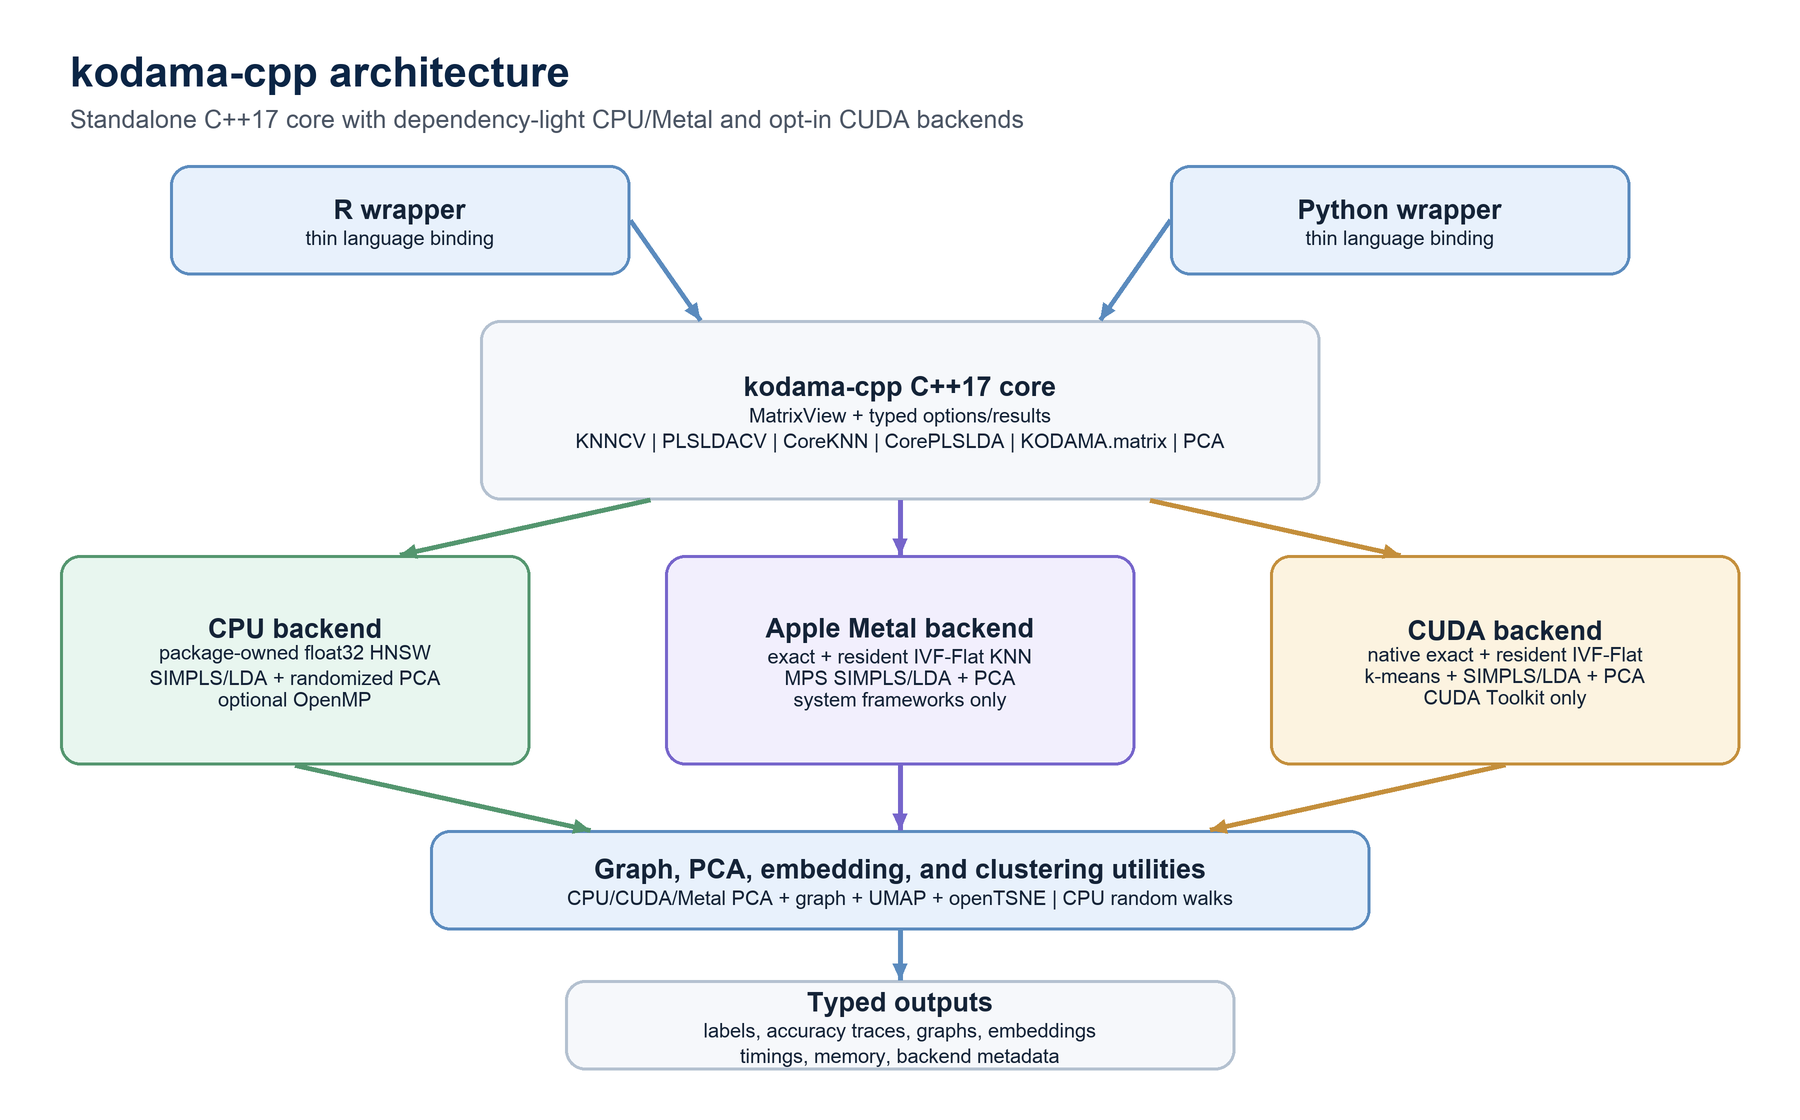
\includegraphics[width=0.92\linewidth]{kodama_cpp_architecture.png}
\caption{The wrapper-independent C++17 core owns numerical state and dispatches to CPU, CUDA, and Metal. R and Python convert host objects but do not reimplement KODAMA mathematics.}
\end{figure}

\subsection{Implementation novelty}
kodama-cpp preserves cross-validated predictability as the KODAMA signal but contributes both a systems redesign and an explicit current search policy. The original R implementation remains the historical reference for accuracy maximization and ensemble construction. In the new library, numerical state previously recreated across wrapper calls is represented once in typed C++ objects and reused across folds, proposal cycles, and independent runs.

Prepared accelerator graphs are represented by opaque shared owners: an R external pointer and a Python capsule. Host index and distance arrays are materialized only when requested. The final graph is corrected in place, so simultaneous base and corrected copies are not retained. Cross-session serialization materializes process-local external handles first.

The backends share mathematical invariants but not source-level execution strategies. KNN uses the same metric and voting rules with different search engines. PLS-LDA uses the same SIMPLS deflation and latent LDA model while each accelerator maps the dominant operations to its own memory and matrix-compute model. This separation avoids benchmark-specific branches inside the classifier and makes CPU/accelerator parity an explicit test target.

The CPU PLS-LDA fold path projects training rows directly into class latent sums and the latent Gram matrix, then projects and scores validation rows without retaining complete score matrices. The randomized SIMPLS refresh remains float32. Its norm reduction preserves the original float result when representable and uses double accumulation only when the squared norm exceeds float32 range; the same representation guard is used by Metal. This restores mathematically feasible fixed-component fits without adding a dataset threshold or changing the two-step power iteration.

Guided evolution is deliberately implemented above the classifier layer. Previous held-out predictions determine sample/group proposals and the class-transition graph; the adaptive schedule determines how many groups may move; and each proposal receives one new CV pass. This is a common scaffold, not a classifier-independent state policy: KNN uses the diversity-guarded score directly, whereas PLS-LDA may add transition coarsening and a fragmentation subtraction before the shared cooling decision. The policy can change stochastic trajectories relative to historical KODAMA without changing the definition of a CV prediction.

\subsection{CUDA backend}
The CUDA path is package-owned and uses only CUDA Toolkit libraries. Input matrices are materialized as contiguous float32 buffers. Exact KNN evaluates the requested metric directly, whereas IVF-Flat builds GPU k-means centroids and inverted lists and selects nprobe from an exact pilot query when recall tuning is enabled. The selected nlist, nprobe, pilot recall, and device id are returned with the result. Exact Lloyd assignment uses a bounded 256 MiB score workspace per independent M lane and batches rows when necessary; every row still evaluates every centroid with the same distance and tie rules. Assignments, centroid sums and counts, empty-cluster repair, list counts, prefix offsets, and row-ID scatter remain on CUDA. A move-only ResidentIVFIndex can retain the input, projection, centroids, offsets, and IDs for subsequent self or external-query calls without a hidden process-global cache.

For PLS-LDA, class labels are encoded compactly and the centered X'Y cross-product is formed from class sums on the GPU, avoiding a dense n-by-K one-hot response. Float32 SIMPLS uses reusable thread-local device workspaces that grow to the required capacity; the unreachable legacy double-precision CPU/CUDA path was removed after the August 2026 audit. Fixed-order class accumulation is followed by separate column-sum and centering kernels, avoiding a read/write race in X'Y centering. Each stream owns a persistent cuBLAS workspace. CUDA computes class latent sums as (X'Y)'W and the latent second moment as W'(X'X)W, so training scores need not be materialized. Validation projection, pooled-covariance correction, Cholesky solve, and LDA scoring remain float32 operations, while fold caches retain train/validation layouts and training Gram matrices.

The default rank-one randomized SIMPLS refresh uses two power iterations. CUDA dispatches the resulting rank-one products as matrix-vector operations and omits the algebraically redundant 1-by-1 block eigensolve. After the first component, the preceding weight is the defined warm start, so the implementation also omits generation of a random vector that would be overwritten before use; this removes launches without changing any SIMPLS value. The multi-vector refresh remains available under the same deflation equations. Latent LDA forms pooled covariance from score and class-sum statistics, retries the trace-normalized ridge sequence only after a failed Cholesky factorization, and copies back predicted codes rather than score matrices.

The CUDA backend uploads the full graph once and keeps per-worker landmark/fold, label, projection, voting, SIMPLS, and LDA allocations alive across independent runs. Values that mathematically change are refreshed in place, and independent runs retain their seeds and proposal trajectories. Landmark selection, proposal decisions, and compact result collection remain host orchestrated, so the manuscript does not claim a fully device-side evolutionary state machine.

\subsection{Apple Metal backend}
The Apple backend is implemented in Objective-C++ on Metal rather than emulating CUDA. A persistent Metal state owns the process-cached device, command queues, and compute pipelines. Device discovery falls back from the system default to enumerated Metal devices, and independent M workers retain separate command queues and float32 workspaces, paralleling CUDA stream lanes. Native kernels implement exact KNN, projected IVF-Flat search, Lloyd k-means assignment and centroid updates, empty-cluster repair, and inverted-list count, prefix, and scatter operations. The same move-only ResidentIVFIndex contract retains Metal input and index buffers across search calls; self-search therefore does not upload the training matrix again.

The Metal PLS-LDA path uses float32 class-label cross-products and the same SIMPLS component limit as CPU and CUDA. Metal Performance Shaders execute the dominant Xw and X't matrix products through MPSMatrixMultiplication. The same two-iteration incremental refresh and SIMPLS loading deflation are used on all three backends; the comparatively small response-space products and deflation updates remain host operations. This division is stated explicitly because a native Metal backend does not imply that every scalar operation is a GPU kernel. Metal materializes projected scores only in a worker-local device buffer, uses a label-aware kernel for class sums and MPS matrix multiplication for T'T, uploads the small fitted LDA model, and returns validation labels after on-device scoring.

Metal is a first-class backend contract: it has named KNNCV, PLSLDACV, CoreKNN, CorePLSLDA, and KODAMAMatrix entry points, reports Metal in result metadata, and is covered by dedicated parity tests. Unsupported Metal operations fail explicitly instead of being relabeled CPU execution. The R integration layer accepts backend = 'metal' explicitly and links the Metal, MetalPerformanceShaders, and Foundation system frameworks without FAISS or cuVS link flags. This makes Apple GPU results auditable in the same manner as CUDA results.

Metal also exposes native fuzzy/binary UMAP and FFT-grid openTSNE while retaining the package-owned graph and backend-native PCA initialization. Following the audited fastEmbedR source, CPU uses a CSR UMAP epoch schedule, CUDA uses an atomic COO/CSR epoch schedule, and Metal uses the clean row sampler with fixed-point atomic coordinate updates. openTSNE retains sparse attractive forces, FFT-grid repulsion, gains, momentum, and centering on Metal. These native paths are exposed consistently in the C++, R, and Python APIs.

\subsection{Shared accelerator contract}
\begin{table}[h]
\caption{Backend contracts retained by the release.}
\footnotesize
\begin{tabularx}{\linewidth}{>{\raggedright\arraybackslash}p{0.18\linewidth}%
  >{\raggedright\arraybackslash}X>{\raggedright\arraybackslash}X>{\raggedright\arraybackslash}X}
\toprule
Contract & CPU & CUDA & Apple Metal \\
\midrule
Internal precision & Contiguous float32 host/device matrices and reusable CUDA buffers. & Float32 shared MTLBuffers and MPSMatrix objects. \\
KNN & Exact or recall-tuned IVF-Flat with device-built lists, returned metadata, and an explicit resident-index owner. & Exact or recall-tuned IVF-Flat with device-built lists and the same resident-index lifetime. \\
PLS-LDA & GPU label cross-products, SIMPLS workspace, projection, class summaries, and LDA scoring. & Label-aware cross-product with MPS-accelerated X projections and shared SIMPLS/LDA semantics. \\
KODAMA evolution & For a fixed classifier: same folds, constrained proposals, classifier-specific score, requested feasible components, and independent M runs. & For a fixed classifier: same folds, constrained proposals, classifier-specific score, requested feasible components, and independent M runs. \\
Failure semantics & Unavailable CUDA entry points throw; no CPU fallback is labeled CUDA. & Unavailable Metal entry points throw; no CPU fallback is labeled Metal. \\
\bottomrule
\end{tabularx}
\end{table}

The public surface groups cross-validation, core optimization, graph preparation, matrix and graph-input KODAMA, PCA, visualization, and graph utilities. In the R ecosystem, numerical PCA and the Louvain, Leiden, and Walktrap wrappers are owned by fastEmbedR. KODAMA's object-aware \texttt{RunFastPCA} adapter delegates to \texttt{fastEmbedR::pca} after selecting and orienting matrix, SingleCellExperiment, SpatialExperiment, Seurat, or Giotto data; it does not maintain a second R-level PCA implementation. Spatial benchmark clustering likewise calls \texttt{fastEmbedR::knn\_graph} and \texttt{fastEmbedR::graph\_cluster}, while KODAMAextra is used only for the established tissue plotting helper. The installed C++ headers and generated R/Python references are the authoritative signature list.

\subsection{Graph-first input contract}
KODAMA.graph returns a matrix- or external-handle-backed graph, backend-matched PCA starts, metadata, and timings, but never the source matrix. Raw features remain caller-owned when supplied separately.

\begin{table}[h]
\caption{Graph-first KODAMA.matrix input contract.}
\small
\begin{tabularx}{\linewidth}{p{0.12\linewidth}X X X p{0.10\linewidth}}
\toprule
Input & Working geometry & KNN evolution & PLS--LDA evolution & Graph builds \\
\midrule
Raw X & Raw float32 variables & Data-native KNN & Raw variables & One \\
Prepared P & Self-tuning graph features & Fixed supplied graph & Laplacian surrogate & Zero \\
Prepared P + X & Raw float32 variables & Fixed supplied graph & Raw variables & Zero \\
Bare G & Self-tuning graph features & Fixed supplied graph & Laplacian surrogate & Zero \\
\bottomrule
\end{tabular}
\end{table}

\begin{scriptsize}
\begin{verbatim}
Algorithm: graph preparation and KODAMA.matrix dispatch

KODAMA.Graph(X, k, backend):
  X32 <- Float32(X)
  G <- BackendKNN(X32, k)
  (Z_U, Z_T) <- BackendPCAStarts(X32)
  return P = {G, Z_U, Z_T, dimensions, backend, timings}
  # X32 and X are not retained by P.

KODAMA.Matrix(input, optional X):
  raw X        -> prepare P; use raw geometry
  prepared P+X -> reuse P; use caller-owned raw geometry
  prepared P   -> reuse P; use self-tuning graph geometry
  bare G       -> use G with no stored PCA starts and graph geometry
\end{verbatim}
\end{scriptsize}

MetRef CUDA smoke validation used n = 873, p = 375, k = 100, and M = T = 10. The prepared R object occupied 1.08 MB and contained no raw-data field, compared with 2.70 MB for the input matrix; one-time graph/PCA preparation required 0.342 wall seconds. Exact PLS-LDA agreement confirms that prepared P does not alter raw-feature classification when X is also supplied. The KNN difference is expected: P + X uses fixed-graph voting, whereas X uses data-native KNN within each landmark sample. P and bare G agree exactly because stored PCA starts affect visualization initialization, not graph-only label evolution. These figures validate API lifecycle semantics and are not presented as a performance benchmark.

\subsection{Computational scaling}
\begin{table}[h]
\caption{Isolated evolution ablations and their single controlled differences.}
\small
\begin{tabularx}{\linewidth}{p{0.18\linewidth}X X}
\toprule
Component & Dominant work & Implementation implication \\
\midrule
KODAMA runs & M independent runs, each with Tcycle proposal cycles plus one initial CV pass. & Embarrassingly parallel over M; each cycle performs exactly one CV evaluation. \\
KNN core & Neighbor search/build plus O(M Tcycle n\_L k) voting on landmarks, where n\_L is the landmark count and k is the KNN predictor size. & Graph-input KNN removes the search/build term and reuses supplied indices and distances. \\
PLS-LDA core & O(M Tcycle folds C\_PLS(n\_train, p, h)) for h requested components, plus latent-space LDA scoring. & Float32 label-aware SIMPLS and fold buffers reduce constants but do not change the repeated-CV structure. \\
Graph correction & O(M E) agreement counting for E retained graph edges, followed by row-wise neighbor sorting. & Sparse by default; dense n by n dissimilarities are avoided for scalability. \\
Visualization & Runs on the base or KODAMA-corrected sparse graph using UMAP/openTSNE helpers. & Visualization time is reported separately because it is not part of the CV optimization objective. \\
\bottomrule
\end{tabularx}
\end{table}

\subsection{Graph-input KODAMA validation boundary}
\begin{table}[h]
\caption{Interpretation of graph-input KODAMA paths.}
\small
\begin{tabularx}{\linewidth}{p{0.18\linewidth}X X}
\toprule
Path & Implementation & Interpretation \\
\midrule
KNN graph input & Uses supplied neighbor indices/distances directly in CoreKNNGraph\_CPU/CUDA/METAL and KODAMAMatrixFromGraph; no neighbor index is rebuilt. & Preserves graph-based KNN voting mathematics. CUDA and Metal upload the supplied graph once and perform fold masking, voting, and prediction with resident graph buffers. \\
PLS-LDA graph input with X & When the original data matrix is supplied with the graph, PLS-LDA uses float32 X and the graph supplies initialization/projection support. & Equivalent classifier path to data-input PLS-LDA; graph handling is an input-format extension. \\
PLS-LDA graph-only input & When X is unavailable, a host kernel transforms the graph into self-tuning normalized Laplacian features before backend-selected CorePLSLDA. & Exposed as an optional spectral surrogate, not as evidence that graph-only PLS-LDA matches data-input PLS-LDA in all datasets. \\
Validation boundary & Wrapper tests exercise both KNN and PLS-LDA graph-input calls; benchmark comparisons must use the same M, Tcycle, seed, and supplied graph. & The manuscript does not use graph-only PLS-LDA results to support data-input KODAMA performance claims. \\
\bottomrule
\end{tabularx}
\end{table}

\subsection{KODAMA directly from a KNN matrix}
The graph-input API represents a KNN matrix as two rectangular arrays with identical shape n by k. Entry I[i,j] is the sample identifier of the jth neighbor of sample i, and D[i,j] is its non-negative dissimilarity. The boundary accepts either zero-based or one-based identifiers, converts them to the internal convention, discards invalid identifiers, self-neighbors, and non-finite distances, clamps negative distances to zero, and retains at most graph.neighbors entries per row. The row order must match the sample order used by every optional label, constraint, and feature vector.

For graph-only KNN KODAMA, the supplied graph replaces construction of the global neighbor index and remains the source of neighbors for CV voting, landmark-label projection, and final agreement correction. A deterministic self-tuning normalized-Laplacian representation is still computed once to provide geometry for landmark selection and initial splitting; it does not replace graph-based KNN voting. If the original data matrix X is available, KODAMAMatrixFromGraphData uses float32 X for that geometry while continuing to reuse the supplied graph.

PLS-LDA requires a rectangular feature representation. With X supplied, graph-input PLS-LDA uses the ordinary float32 SIMPLS plus latent-space LDA classifier on X. With only I and D supplied, it uses the deterministic self-tuning normalized-Laplacian features described above. This graph-only PLS-LDA route is an explicit spectral surrogate and is not claimed to be numerically equivalent to data-input PLS-LDA. Graph normalization and spectral feature extraction are host operations in the current release; CPU, CUDA, or Metal is then selected for the PLS-LDA evolution.

The remaining KODAMA procedure is unchanged: each of M independent runs selects landmarks, initializes at most splitting classes, performs Tcycle proposal and CV updates, and projects its optimized labels to all samples. The output contains the M by n label matrix, one best raw CV accuracy per run, one graph in either base or KODAMA-corrected state, timing fields including graph-feature time, and backend metadata. UMAP or openTSNE can then consume the corrected graph directly; when X is unavailable, visualization reports its graph-only initialization fallback.

The R and Python graph-input functions expose the same contract. Python uses the direct snake\_case transliteration of dotted R names. Defaults, accepted values, the one-based best-run convention, and returned fields are otherwise aligned.

Executable C++, R, and Python calls for every input form are maintained in the public API tutorial so that wrapper syntax does not duplicate the mathematical contract in the publication supplement.

\section{Relationship to public KODAMA literature}
The contribution of kodama-cpp is not a new definition of KODAMA. It is a reorganization of the published method into a reusable numerical system. The 2014 PNAS paper is the methodological reference for accuracy maximization. The 2017 Bioinformatics paper is the software reference for the R package, including KNN and PLS-DA classifiers, repeated suboptimal runs, and construction of a dissimilarity matrix from the optimized label vectors. The R documentation is the public reference for defaults such as M = 100, Tcycle = 20, 75\% sample selection, and the output fields dissimilarity, accuracy, proximity, classification vectors, scores, entropy, and landmarks.

The main differences are architectural and computational. The R package owns a complete R workflow and uses R-package dependencies for data handling, nearest neighbors, and visualization. kodama-cpp owns the numerical kernels and exposes them through C++ types so that R and Python wrappers can share one backend. This makes comparison with the KODAMA R 2.4.1/2.4 predecessor a compatibility question: held-out label predictability remains the central signal and the output roles can be mapped, while exact trajectories need not match because the current standard adds grouped adaptive proposals, transition-driven coarsening, and a disclosed degeneracy guard. Float32 storage, package-owned CPU/CUDA/Metal search, accelerator kernels, and wrapper-independent graph objects are additional implementation changes.

The PLS routes must not be conflated. KODAMA R 2.4.1 exposes its historical PLS-DA decoder. kodama-cpp introduces label-aware SIMPLS followed by LDA in the requested-component latent space, with fixed component-count semantics and native float32 CPU, CUDA, and Metal execution. The MetRef evaluation therefore reports historical PLS-DA quantitatively, but treats it as a contextual predecessor rather than a classifier-matched implementation baseline.

All predecessor performance comparisons in this article use KODAMA R 2.4.1/2.4; later KODAMA releases are excluded from timing, quality, and methodological comparisons. Optional R wrapper utilities are documented separately and are not part of the predecessor performance or quality comparison.

\begin{table}[h]
\caption{Compatibility with the public KODAMA R interface and literature.}
\small
\begin{tabularx}{\linewidth}{p{0.17\linewidth}X X}
\toprule
Aspect & Public R/literature contract & kodama-cpp \\
\midrule
Objective & KODAMA maximizes cross-validated accuracy of an evolving label vector. & Held-out label predictability remains the classifier signal and raw accuracy is reported; the standard search ranks proposals with a disclosed label-only degeneracy guard. \\
Search dynamics & The historical core evolves labels through its published stochastic accuracy-maximization procedure. & Grouped adaptive moves and transition-driven coarsening are explicit search extensions; they use CV predictions but never reference labels. \\
Independent runs & R documentation reports M iterative processes and Tcycle optimization cycles. & KODAMAMatrixOptions exposes runs and cycles; runs remain independent across CPU, CUDA, and Metal backends. \\
Sample selection & The documented FUN\_SAM default selects 75\% of samples per iterative process. & Landmark and splitting controls preserve the same sampling role while exposing it in typed options. \\
Classifiers & The R package documents KNN and PLS-DA classifiers. & The KODAMA optimizer exposes KNN and SIMPLS + PLS-LDA; component count is explicit. \\
Output contract & The R interface returns dissimilarity, accuracy, proximity, label vectors, scores, entropy, and landmarks. & The C++ result returns optimized labels, accuracies, graphs, timings, memory, and backend metadata for wrappers. \\
Architecture & The R package is built around R workflows and R dependencies. & The core is R/Python independent, CMake-installable, and accelerated where available. \\
\bottomrule
\end{tabularx}
\end{table}

\subsection{Relationship to semi-supervised learning and cluster validation}
KODAMA is related to, but distinct from, semi-supervised learning and weak supervision. Classical semi-supervised graph methods assume that at least some labels are observed and then propagate them under smoothness assumptions, as in Gaussian-field label propagation and local-global consistency. Pseudo-labeling and weak-supervision systems also create or aggregate imperfect labels, but they typically use those labels to train a downstream predictor. KODAMA reverses the emphasis: the label vector itself is the optimization object, and its quality is the ability of a chosen classifier to reproduce it under held-out folds.

The closest evaluation literature is cluster validation by stability or prediction. Methods such as stability-based clustering and prediction strength ask whether a grouping is reproducible under perturbation or held-out prediction. KODAMA uses the same general principle of reproducibility, but internalizes it as the search objective over label vectors. This is why the benchmark reports the internal CV score together with adjusted Rand index, silhouette, local purity, and active class count rather than presenting CV accuracy alone as proof of external correctness.

The manuscript also follows warnings from the model-selection and circular-analysis literature. Cross-validation can be biased when the same data are used both to choose a model and to estimate final performance; feature selection outside the resampling loop is a classic example. In kodama-cpp, the internal CV score is intentionally the search criterion, so external claims must come from separate diagnostics, transparent parameter sensitivity, and comparisons with standard UMAP and t-SNE on the same datasets.

\begin{table}[h]
\caption{Literature positioning of KODAMA.}
\small
\begin{tabularx}{\linewidth}{p{0.22\linewidth}X X}
\toprule
Literature area & Typical goal & Role of KODAMA \\
\midrule
Semi-supervised graph learning & Label propagation and local-global consistency start from observed labels and smooth them on a graph. & KODAMA starts from synthetic or supplied candidate labels and optimizes their cross-validated predictability. \\
Pseudo-labeling and weak supervision & Pseudo-labeling and data programming create imperfect labels to train predictive models. & KODAMA treats the label vector as the object being discovered; the classifier is the measuring instrument. \\
Cluster stability and prediction strength & Stability methods evaluate whether clusters survive perturbation or prediction on held-out samples. & KODAMA turns held-out predictability into an optimization objective, then reports external diagnostics separately. \\
Manifold visualization & UMAP and t-SNE optimize low-dimensional layouts from neighbor or affinity structures. & KODAMA supplies a corrected graph to the same visualization step; it does not replace those embedding objectives. \\
Open-source ML software & JMLR software papers emphasize clear APIs, reproducibility, tests, licensing, and benchmark transparency. & kodama-cpp separates the numerical core from R/Python wrappers and records backend parameters and validation evidence. \\
\bottomrule
\end{tabularx}
\end{table}

\section{Evaluation}
We evaluate kodama-cpp at three levels. First, kernel benchmarks isolate KNNCV and PLSLDACV from the full KODAMA matrix pipeline so that nearest-neighbor search and PLS-LDA fitting can be interpreted separately. Second, core optimizer benchmarks measure repeated label-vector evolution over multiple seeds. Third, matrix-level validation measures end-to-end KODAMA.matrix calls and reports both cross-validated accuracy and external-label diagnostics where reference labels are available.

The evaluation is intentionally separated into these layers because KODAMA has several scaling regimes. KNN acceleration is dominated by neighbor search and voting. PLS-LDA acceleration is dominated by repeated SIMPLS and LDA work across folds and cycles. The final graph and visualization stages depend primarily on the sparse graph size. Reporting the layers separately makes it possible to attribute a speedup to the part of the implementation that produced it.

The evaluation also separates optimization from validation. Held-out CV accuracy is the internal classifier signal, while the current standard ranks proposals with the disclosed label-only acceptance score. Neither quantity is interpreted as external biological, chemical, or semantic truth. When reference labels are available, they are held outside the optimizer and reported after the fact. This distinction follows the broader cautionary literature on model selection, feature selection bias, and circular analysis.

All timings in this section are wall-clock seconds from the benchmark drivers, and all accuracy values are computed on held-out cross-validation folds. CPU kernel measurements use the configured single-thread CPU path unless explicitly labeled otherwise; CUDA measurements use the same CUDA Toolkit runtime used by the test suite. Tables are intentionally separated by scope: kernel-level rows do not claim end-to-end speedups, and graph-input rows are treated as API validation unless paired with data-input KODAMA results under the same M, Tcycle, seed, and graph settings.

\subsection{Audited implementation improvements}
Accepted changes preserve the KODAMA objective while correcting fold isolation, index-base ownership, float32 numerical range, graph residency, repeated fold work, and wrapper conversion. CPU streams PLS-LDA sufficient statistics; CUDA derives them from resident class sums and fold Gram matrices; Metal now uses a label-aware class-sum kernel, MPS T'T, and on-device validation scoring. Leakage, numerical, backend, and wrapper regressions cover these contracts. The dated repository audit maps every claim to source, tests, and retained benchmark files.

\subsection{Benchmark protocol and data coverage}
\begin{table}[h]
\caption{Benchmark protocol for the current evaluation.}
\begin{tabularx}{\linewidth}{p{0.22\linewidth}X}
\toprule
Variant & Only change relative to full standard KODAMA \\
\midrule
Date & 2026-07-27 UTC for the matched current-commit MetRef CPU/CUDA run; earlier validation snapshots are dated explicitly \\
GPU & NVIDIA GeForce RTX 5060 Ti, 16 GB device memory, driver 595.71.05 \\
Build validation & Fresh CUDA 13.0 compute-capability-12.0 build at 9da48ee succeeded; CTest passed 3/3 and the installed R wrapper passed testthat \\
Runtime & CUDA Toolkit only for native search/PLS paths; no FAISS, cuVS, RAFT, RMM, or Armadillo link \\
Data format & RData lists exported to contiguous float32 row-major matrices \\
CPU setting & Four CPU threads for the matched MetRef end-to-end run; other tables state their worker count \\
Timing boundary & End-to-end wall time starts immediately before the public call and stops after synchronized return, including allocations and host/device transfers; no warm-up is removed unless a row is explicitly labeled microbenchmark \\
CV kernels & KNNCV and PLSLDACV measured independently from the full matrix pipeline \\
Core optimizer & Three seeds per dataset for CoreKNN and CorePLSLDA medians \\
Reported metrics & Wall time, peak memory where available, CV accuracy, ARI, and active class count \\
\bottomrule
\end{tabularx}
\end{table}

\subsection{Evaluation guardrails and ablations}
CV accuracy is the internal search objective, never an external truth score. ARI, silhouette, trustworthiness, local purity, and active-class count are computed only after optimization. Classic and KODAMA embeddings are paired by dataset and seed, timing stages are reported separately, and failures remain explicit. The frozen release protocol predeclares comparisons for search evolution, classifier, graph correction, Tcycle, M, landmark/splitting controls, backend, and wrapper parity; the complete ablation matrix is archived with the benchmark driver.

\subsection{Dependency-free CPU and Apple Metal validation}
The dependency-light backend experiment was run on macOS with CUDA and OpenMP disabled. The CPU build therefore measures the package-owned HNSW and float32 SIMPLS/LDA implementations, while the Metal build links only Apple system frameworks. CPU/Metal agreement within the documented float32 tolerance is the primary acceptance criterion; timings are secondary evidence. A historical MetRef KNNCV diagnostic reporting 11.145 versus 0.026 seconds lacked a retained warm-up and synchronization record and has therefore been removed from the quantitative table rather than defended as a 425-fold speedup.

A focused Apple M3 graph benchmark used 4,000 samples, 32 float32 variables, k = 30, and three repeated runs. Before concurrent insertion, the accepted implementation builds a deterministic connected seed containing min(n, max(n\_threads + 1, 2 m\_HNSW + 1)) points, where m\_HNSW is the internal graph connectivity. Parallel HNSW construction required a median 6.722 s with one thread and 1.791 s with four threads, a 3.75-fold scaling gain. The earlier four-thread serial-insertion implementation required 7.248 s, so the accepted implementation was 4.05-fold faster. Four-thread overlap with the one-thread graph had a three-run median of 0.99966. Across 100 repeated four-thread builds of a 600 by 24 test problem with k = 20, minimum and mean brute-force recall were 0.99975 and 0.99987. Both serial and parallel paths must retain at least 0.99 exact-neighbor recall in CTest, and the complete CPU suite passes ThreadSanitizer.

The portable float32 distance loop is structured for compiler vectorization; Apple Clang emits 128-bit NEON arithmetic without a separate architecture path. On x86-64, a one-time per-index capability check selects a package-owned 256-bit AVX2/FMA kernel when supported and otherwise retains the portable loop. On an Intel Core i7-13700, five-run medians for the same 4,000 by 32, k = 30 benchmark decreased from 1.342554 to 1.253022 seconds with one thread and from 0.362764 to 0.337393 seconds with four threads. Candidate single-thread/four-thread graph overlap was 1.000 in all five runs. Explicit software prefetching was rejected after neutral-to-negative timings. HNSW candidate heaps were already reserved per worker, and final CPU graph correction now similarly reuses one sorting buffer per OpenMP worker; the latter preserved the exact result hash and had essentially neutral wall time.

Metal IVF-Flat remains an explicit option rather than an automatic replacement for exact search. On MNIST10k, exact and recall-tuned IVF KNNCV both produced accuracy 0.9490, while elapsed time changed from 2.054 to 1.662 s. A 0.99 pilot-recall target was rejected because accuracy decreased to 0.9482; the accepted automatic pilot target is 0.999. End-to-end KODAMA can still favor exact search when repeated IVF training costs more than the saved query time.

A 7 August 2026 local worktree screen provides preliminary crossover evidence, not release-tagged confirmatory results. One CPU graph per dataset and seed was supplied unchanged to CPU4 and Metal, separating optimizer timing from backend-specific graph search. Across seeds 4, 17, and 42 at M = 20 and Tcycle = 20, median Metal speedups were 1.79x for MetRef KNN, 1.91x for COIL20 KNN, 2.02x for USPS KNN, and 2.33x for USPS PLS-LDA. MetRef PLS-LDA was effectively tied at 0.98x (25.842 seconds CPU4 versus 26.292 seconds Metal). Median Metal-minus-CPU truth-silhouette changes were +0.0035, +0.0009, -0.0002, +0.0036, and -0.0044 for those five cells, respectively. Raw-variable COIL20 PLS-LDA at 50 components was stopped after more than 600 seconds before one independent run completed; the paired Metal cell was not started. Both outcomes are retained as censored local feasibility evidence rather than replaced by PCA or a smaller component count. A separate bounded M=4/Tcycle=1 scheduler study found identical CV and ARI summaries for one through four Metal lanes, with optimization times 61.578, 38.685, 47.883, and 40.856 seconds, respectively. Because back-to-back GPU timing was sensitive to thermal and run order, the accepted automatic planner uses retained CV-fold bytes and the Metal working-set budget rather than choosing the fastest row. It selected three lanes for COIL20 and four for MetRef on the tested 8 GB Apple M3.

A full-cycle follow-up used one unchanged CPU HNSW graph and the same CPU UMAP backend for CPU4 and physical Metal at M = 100 and Tcycle = 100. On USPS, Metal reduced KNN optimization from 12.451 to 7.888 seconds (1.58x) and pipeline time from 15.480 to 10.972 seconds, while truth-label silhouette was 0.4550/0.4555. PLS-LDA showed the opposite systems result: CPU4 required 707.057 seconds and Metal 1105.998 seconds, with truth-label silhouette 0.4227/0.4174. Classic UMAP silhouette was approximately 0.13. Together with full-cycle MetRef, this demonstrates a classifier- and matrix-shape crossover rather than universal accelerator speedup. The local worktree was dirty, so these rows are engineering controls awaiting clean tagged CPU4/CUDA replication.

A third full-cycle control used ImageSegmentation (2,310 by 19; seven withheld truth classes), one unchanged CPU graph, CPU UMAP, seed 4, and M = Tcycle = 100. KNN optimization required 1.107 seconds on CPU4 and 1.672 seconds on Metal; truth-label silhouette was 0.5387 and 0.5396, versus 0.2935 and 0.2956 for classic UMAP. PLS-LDA required 12.557 seconds on CPU4 and 125.108 seconds on Metal; silhouette was 0.6418 and 0.6503. The requested 50 PLS components were correctly limited to the 19 mathematically feasible components. This negative accelerator result reinforces that backend advantage depends on matrix shape; Metal execution is validated but is not claimed to be universally faster.

A fourth full-cycle control used PageBlocks (5,473 by 10; five strongly imbalanced truth classes), the same shared-graph design, seed 4, and M = Tcycle = 100. CPU4/Metal KNN optimization required 2.778/2.722 seconds and median CV accuracy was 0.99683/0.99732. CPU4/Metal PLS-LDA required 13.655/118.383 seconds while median CV accuracy remained close at 0.90512/0.90524. Classic and KODAMA truth silhouettes were all negative; the dataset is therefore retained as a backend-parity and adverse-quality control, not as evidence of visualization improvement. It also establishes a low-dimensional regime in which physical Metal PLS-LDA is substantially slower than CPU4.

A fifth full-cycle control used PenDigits (10,992 by 16; ten withheld truth classes), the same shared-graph design, seed 4, and M = Tcycle = 100. CPU4/Metal KNN optimization required 4.397/4.925 seconds with median CV accuracy 0.99672/0.99588. CPU4/Metal PLS-LDA required 39.311/199.897 seconds with median CV accuracy 0.97198/0.97350. In contrast to the high internal scores, classic UMAP truth-label silhouette was 0.5116 and every KODAMA silhouette was negative (-0.0832 to -0.1009). The diffuse plots are retained as an adverse ensemble-correction result: CV accuracy is not an external-label objective, and a fragmented label ensemble can weaken the corrected graph. No dataset-specific parameter change was accepted.

A sixth local stress control used raw COIL20 (1,440 by 16,384; 20 withheld truth classes), seed 4, M = Tcycle = 100, and 1,080 effective landmarks under the unchanged 75\% rule. CPU4/Metal KNN optimization wall time was 193.377/80.753 seconds, a 2.39x Metal speedup, and median CV accuracy was 0.99537 on both backends. Complete pipeline time was 200.950/88.315 seconds. Both KODAMA truth silhouettes (0.4531/0.4278) were below classic UMAP (0.5266/0.5303), so this is acceleration and adverse-quality evidence, not a universal improvement claim. Raw CPU4 PLS-LDA exceeded 300 seconds before the first four independent runs completed and is retained as a censored resource-limit cell.

A seventh local control used SatImage (6,435 by 36; six withheld truth classes), seed 4, M = Tcycle = 100, and 4,827 effective landmarks. The initial implementation required 3.044/3.216 seconds for CPU4/Metal KNN and 56.540/331.781 seconds for PLS-LDA. A backend lifecycle audit then replaced one-slot Metal fold residency with a bounded 16-entry LRU and made independent-run concurrency memory-aware. With the same serialized CPU graph, seed, and mathematics, corrected CPU4/Metal times were 2.963/2.442 seconds for KNN and 56.484/171.675 seconds for PLS-LDA. Metal therefore became 1.21x faster for KNN and 1.93x faster than its own pre-fix PLS-LDA path, although low-dimensional PLS-LDA remained 3.04x slower than CPU4. Median CV accuracy remained closely matched (KNN 0.99834/0.99772; PLS-LDA 0.94883/0.94893), no run collapsed, and PLS-LDA selected-label ARI was 0.493/0.581. KODAMA truth-label silhouettes remained below classic UMAP, so this is lifecycle and crossover evidence rather than a universal visualization-improvement claim.

A subsequent fold-identity audit found that sequential Metal PLSLDACV calls without a persistent fold cache could reuse a temporary host address and incorrectly retain the previous fold matrix. Fold-specific worker-local residency epochs corrected the issue without changing SIMPLS or LDA. On raw COIL20 with five folds, 20 components, and 16,384 predictors, one-worker accuracy increased from the erroneous 0.555556 to 0.959028 and then matched four workers across seeds 4, 17, and 42. Median one/four-worker kernel times were 0.634/0.406 seconds. In a nested predictor-width study, median four-core CPU/Metal kernel speedups were 1.71x, 5.19x, 13.82x, and 10.78x at 256, 1,024, 4,096, and 16,384 predictors. These results characterize the kernel crossover; they do not remove the much larger cost of a complete M-by-Tcycle high-dimensional KODAMA search. A later lifecycle audit extended the identity rule across calls: uncached stratified invocations now receive a fresh residency generation, while fixed non-stratified KODAMA folds retain stable cache generations. A sequential changed-label regression reproduces CPU fold assignments, predictions, and accuracy on physical Metal.

A preserved-executable follow-up evaluated streamed CPU LDA sufficient statistics with five folds, 50 fixed components, four workers, seed 7, and three fresh processes. Predictions and accuracy were identical on MetRef, USPS, COIL20, and TabulaMuris. TabulaMuris (100,102 by 50) improved from 4.110 to 2.794 seconds (1.47x), and the reported peak-memory ratio was 0.587. Full MetRef KODAMA at M=5 and Tcycle=5 retained best CV 0.854962, ARI 0.590789, and 55 classes while median CPU time improved from 1.659 to 1.611 seconds.

Full MNIST70k then exposed a float32 range failure in the randomized SIMPLS norm rather than a rank limitation: the former CPU path returned a one-component majority fallback at accuracy 0.112529, and Metal failed. An overflow-only norm fallback restored all 50 requested components at accuracy 0.866457 on CPU and 0.866286 on Metal; median Metal time was 2.296 seconds across three fresh processes. MetRef, COIL20, and TabulaMuris accuracies were unchanged; Metal USPS improved by six predictions among 11,000 samples. A compact synthetic regression passes normal CPU tests, AddressSanitizer, and the physical Metal suite. These local worktree results require confirmation on the frozen CUDA tag before they become release evidence.

A subsequent Metal PLS-LDA transfer audit retained MPS projection on-device, reduced training scores to class sums with a label-aware kernel, formed T'T with MPS matrix multiplication, and scored validation rows on Metal. Complete projected score matrices no longer return to the host; the small fitted LDA model is uploaded and only final integer labels return after validation scoring. The device score buffer, SIMPLS fit, LDA covariance, ridge sequence, priors, and component count are unchanged. A direct regression reproduces the former host calculation from the same projected scores. In three-process seed-7 comparisons, accuracy and 50 selected components were unchanged on five datasets. Metal PLSLDACV improved from 1.799 to 0.492 seconds on TabulaMuris (3.65x) and from 2.296 to 1.704 seconds on MNIST70k (1.35x), was 1.14x faster on USPS, neutral on raw COIL20, and 0.94x on tiny MetRef. A three-seed CPU4/Metal screen retained a maximum absolute accuracy difference of 0.001145. A follow-up replaced the serial-per-component-pair T'T kernel with the MPS product. Across three alternating-order seed pairs, median paired speedups were 1.14x on TabulaMuris and 1.10x on MNIST70k with 50 components and no PLSLDACV accuracy decrease; seven-repeat checks gave 1.13x and 1.01x. Tiny MetRef was 0.99x. These are local worktree engineering results, not frozen release claims.

A later full-cycle Metal lifecycle audit identified two orchestration defects rather than a classifier limitation. A single-slot resident matrix cache repeatedly evicted the immutable five-fold matrices, and the independent-M scheduler was capped at four lanes irrespective of the device working-set budget. A bounded 16-entry least-recently-used fold cache and a device-budgeted scheduler of at most 32 lanes preserve the SIMPLS, LDA, proposal, and temperature equations. At M = Tcycle = 100, MetRef PLS-LDA improved from 631.415 to 312.029 seconds (26 selected lanes), versus 316.329 seconds on four CPU cores. Best CV accuracy 1.000000, selected ARI 0.860185, 32 selected classes, median 25 classes, range 16--35, and zero collapse rate were unchanged. The rejected resident predictor-Gram experiment is not present in the implementation.

Three in-process MetRef Metal graph calls required 0.136, 0.023, and 0.023 seconds wall time, showing that the small-data first-use difference is one-time pipeline compilation; the four-core CPU graph required 0.152 seconds.

A standalone Metal UMAP follow-up supplied one identical CPU graph and PCA start to the CPU and Metal optimizers for 200 epochs. Warm Metal speedups were 1.08x on MetRef, 6.10x on USPS, and 6.52x on TabulaMuris; truth-label edge agreement@15 was 0.6225/0.6309, 0.7077/0.7084, and 0.8828/0.8828 for CPU/Metal. Against a current fastEmbedR source snapshot, fuzzy-graph edge counts and maximum weights matched exactly on all three datasets. Physical C++, R, and Python Metal tests pass. A subsequent native Metal openTSNE validation used matched graphs and PCA starts on MetRef, USPS, and full TabulaMuris. KODAMA/fastEmbedR Metal openTSNE pair-distance correlations were 0.9863, 0.9981, and 0.9928, while KODAMA Metal/CPU correlations were 1.0000, 0.9997, and 0.9990. A later audit of fastEmbedR main at 5248ee0 found no changed native UMAP optimizer file and an identical SHA-256 for the complete exported float32 openTSNE function relative to the pinned parity snapshot; unrelated R-control, PCA, and graph-clustering additions were not copied. Warm KODAMA Metal times were 0.054, 0.201, and 0.556 seconds. These are local worktree results.

A full local MetRef comparison then used one shared CPU graph, seed 4, 655 effective landmarks, M = 100, Tcycle = 100, 50 requested PLS components, and identical CPU UMAP visualization. CPU4/Metal KNN optimization required 2.729/1.609 seconds and produced truth-label silhouettes 0.3293/0.3333, but both selected two classes and had low ARI (0.0430/0.0472). CPU4/Metal PLS-LDA optimization initially required 335.734/651.767 seconds, while best CV accuracy was 1.000 for both and median CV accuracy was 0.993893 for both. A single-lane Metal follow-up was stopped after two runs required 46.8 seconds and was rejected. Later lifecycle and resident-workspace corrections reduced the accepted Metal result to 273.013 seconds. A final automatic-scheduler run selected 26 independent resident M workers from the Metal working-set budget and required 263.568 seconds (3.46\% faster), with best/median CV accuracy 1.000/0.993893, best ARI 0.860185, median 25 classes, no runs with two or fewer classes, and KODAMA UMAP truth silhouette 0.833023. Fully device-native SIMPLS, a fused MPS recurrence, and private fold-buffer prototypes were separately tested, found slower at publication-scale Tcycle, and removed. No dataset-specific scheduling rule or mathematical change was accepted.

\begin{table}[h]
\caption{Dependency-free CPU and native Apple Metal validation. Quality entries are CPU/Metal where two values are shown.}
\small
\footnotesize
\begin{tabularx}{\linewidth}{@{}p{0.08\linewidth}p{0.18\linewidth}p{0.08\linewidth}p{0.08\linewidth}p{0.08\linewidth}X@{}}
\toprule
Dataset & Scope & CPU s & Metal s & Speedup & Quality \\
\midrule
MetRef & PLSLDACV, 50 components, five-run median & 0.790 & 0.202 & 3.90x & accuracy 0.990836 / 0.989691 \\
MetRef & KODAMA KNN, M=10 T=20 & 21.709 & 0.171 & 127x & CV 0.978626; ARI 0.093922; 15 classes \\
MetRef & KODAMA PLS-LDA, M=8 T=20 & 14.930 & 6.900 & 2.16x & best CV 0.963359 / 0.969466; ARI 0.741026 / 0.849732 \\
MetRef & KODAMA KNN, M=100 T=100, shared graph & 2.729 & 1.609 & 1.70x & best CV 1.000 / 1.000; two classes \\
MetRef & KODAMA PLS-LDA, M=100 T=100, corrected shared graph & 316.329 & 312.029 & 1.01x & median CV 0.993893 / 0.993893; selected ARI 0.860185; no collapse \\
USPS & KODAMA KNN, M=100 T=100, shared graph & 12.451 & 7.888 & 1.58x & median CV 0.99333 / 0.99345; sil. 0.4550 / 0.4555 \\
USPS & KODAMA PLS-LDA, M=100 T=100, shared graph & 707.057 & 1105.998 & 0.64x & median CV 0.95376 / 0.95370; sil. 0.4227 / 0.4174 \\
Image Seg. & KODAMA KNN, M=100 T=100, shared graph & 1.107 & 1.672 & 0.66x & median CV 0.99596 / 0.99481; sil. 0.5387 / 0.5396 \\
Image Seg. & KODAMA PLS-LDA, M=100 T=100, shared graph & 12.557 & 125.108 & 0.10x & median CV 0.97346 / 0.97259; sil. 0.6418 / 0.6503 \\
Page Blocks & KODAMA KNN, M=100 T=100, shared graph & 2.778 & 2.722 & 1.02x & median CV 0.99683 / 0.99732; sil. -0.1627 / -0.1802 \\
Page Blocks & KODAMA PLS-LDA, M=100 T=100, shared graph & 13.655 & 118.383 & 0.12x & median CV 0.90512 / 0.90524; sil. -0.1835 / -0.1694 \\
SatImage & KODAMA KNN, M=100 T=100, corrected shared graph & 2.963 & 2.442 & 1.21x & median CV 0.99834 / 0.99772; no collapse \\
SatImage & KODAMA PLS-LDA, M=100 T=100, corrected shared graph & 56.484 & 171.675 & 0.33x & median CV 0.94883 / 0.94893; ARI 0.493 / 0.581 \\
\bottomrule
\end{tabularx}
\end{table}

\subsection{CUDA workstation validation}
The benchmark corpus uses copied float32 RData datasets spanning n = 873 to 5,220,347 samples and p = 11 to 16,384 variables. For the current matched MetRef result, commit 9da48ee was rebuilt with CUDA 13.0 for compute capability 12.0; all three configured CTest targets and the installed R-wrapper testthat suite passed. Broader tables retain explicitly dated release-history snapshots rather than silently mixing them with this current-commit run.

The current package-owned CUDA IVF-Flat path was checked on MNIST70k and MetRef with five-fold cosine KNNCV and k = 10. On MNIST70k it produced accuracy 0.973857 in 4.233 s with nlist = 237 and maximum nprobe = 32, compared with 0.973029 in 4.753 s for the recorded former FAISS/cuVS row. On MetRef it produced 0.816724 in 0.195 s, compared with 0.814433 in 0.297 s. These are implementation spot checks rather than repeated-run performance estimates.

A focused resident-IVF microbenchmark separated construction from repeated search on a deterministic 50,000 by 32 float32 matrix using five timed searches after one warm-up. For all-row self-search, retaining the index reduced mean rebuild-plus-search time from 0.8695 to 0.8091 s on Metal and from 0.1984 to 0.1765 s on CUDA (1.07x and 1.12x). For 1,000-query batches against the same training matrix, time changed from 0.1179 to 0.0306 s on Metal and from 0.0318 to 0.0092 s on CUDA (3.86x and 3.45x). Neighbor overlap was 1.000 in every comparison. These are systems measurements, not dataset-level accuracy estimates.

The current M = 100, Tcycle = 100 MetRef validation shows why cross-validated accuracy is reported together with label-quality diagnostics. Matched CPU and CUDA PLS-LDA runs both reached maximum CV accuracy 1.000 and median CV accuracy 0.992366. Their CV-selected runs contained 24/27 classes and attained ARI 0.7654/0.7732 against 22 withheld reference classes. Backend-native k = 30 fuzzy UMAP produced truth-label silhouette 0.8206/0.7856. Because finite-precision and scheduling differences can select different stochastic runs, these results support matched objective behavior rather than bitwise trajectory identity.

The dependency-distilled CUDA build links CUDA Toolkit libraries but no FAISS, cuVS, RAFT, or RMM soname. Binary wrappers therefore need to locate the CUDA runtime selected at build time, but do not need to provision the removed search libraries.

The exact-quota selector was also isolated on flow18 (1,000,021 rows, 11 variables). With a request exceeding n, the historical rule yielded 750,016 effective landmarks. Matrix-only sampling from 300 coarse strata required 0.321 seconds and represented all 300 strata. An earlier exact-search CUDA KNN run with M = 1 and Tcycle = 10 required 362.348 seconds, including 335.079 seconds for the shared 100-neighbor graph. This diagnosis motivated automatic accelerator graph dispatch. In the accepted resident implementation, graph time fell from the matched 296.482-second exact baseline to 25.938 seconds (11.43x). At M = 100, Tcycle = 100, and 1,000 landmarks, graph-returning KNN and PLS-LDA required 47.358 and 66.135 seconds; labels-only execution required 46.945 and 64.987 seconds because it omitted the final host graph download. Best CV accuracy remained 1.000 for both classifiers; PLS-LDA ARI changed from 0.926970 to 0.924996 between exact and IVF search and was unchanged by residency.

\begin{table}[h]
\caption{Dependency-distilled native CUDA KNN spot checks.}
\small
\begin{tabular}{lllllll}
\toprule
Dataset & Path & Accuracy & Seconds & nlist & max nprobe & Pilot recall \\
\midrule
MNIST70k & native IVF-Flat & 0.973857 & 4.233 & 237 & 32 & 0.994531 \\
MetRef & native IVF-Flat & 0.816724 & 0.195 & 27 & 20 & 0.991406 \\
\bottomrule
\end{tabular}
\end{table}

\subsubsection{Archived kernel and core diagnostics}
Earlier kernel-only and core-optimizer measurements are retained in the benchmark archive for release-history continuity. They are not repeated here because they use different timing boundaries from the native end-to-end and shared-graph comparisons below. Their seed-level outputs remain available for audit.

For one edge, the worst-case Monte Carlo standard error of an agreement proportion is $1/(2\sqrt M)$: 0.1118 at $M=20$, 0.0707 at $M=50$, and 0.0500 at $M=100$. In the retained MetRef/USPS study, M50 agreement correlations with M100 were 0.9888--0.9988. $M=100$ is retained to control ensemble uncertainty, not to maximize an externally labelled score.

\begin{table}[h]
\caption{Agreement-graph convergence relative to $M=100$.}
\small
\begin{tabular}{llcc}
\toprule
Dataset & Classifier & Backend & Seconds & CV acc & ARI & Classes & Scope \\
\midrule
MetRef & KNN & CPU & 0.147 & 0.963 & 0.271 & 16 & core optimizer \\
MetRef & KNN & CUDA & 0.122 & 0.947 & 0.313 & 16 & core optimizer \\
MetRef & PLS-LDA & CPU & 16.597 & 0.885 & 0.357 & 53 & core optimizer \\
MetRef & PLS-LDA & CUDA & 0.626 & 0.838 & 0.366 & 48 & core optimizer \\
USPS & KNN & CPU & 2.282 & 0.969 & 0.216 & 59 & core optimizer \\
USPS & KNN & CUDA & 0.242 & 0.968 & 0.240 & 53 & core optimizer \\
USPS & PLS-LDA & CPU & 20.189 & 0.938 & 0.140 & 80 & core optimizer \\
USPS & PLS-LDA & CUDA & 1.950 & 0.910 & 0.146 & 77 & core optimizer \\
\bottomrule
\end{tabular}%
}
\end{table}

\subsubsection{KODAMA 2.4.1/2.4 predecessor comparison}
A KODAMA 2.4.1/2.4 KNN-compatible predecessor experiment used MetRef, KNN, M = 100, Tcycle = 100, 655 effective landmarks under the historical 75\% rule, splitting = 50, k = 30, graph k = 100, and seed 1234. Splitting = 50 matches the internal k-means initialization in KODAMA R 2.4.1. KODAMA R 2.4.1/2.4 is the designated and sole predecessor performance baseline. KNN provides the classifier-matched systems comparison. Historical PLS-DA is also measured below as a contextual predecessor baseline, but it is not used to calculate a classifier-matched speedup against current SIMPLS plus latent-space LDA. These are single-run preliminary measurements from the retained 16 July archive, not final replicated release estimates.

The current grouped and guarded proposals extend the historical stochastic search, so this is a matched-settings predecessor and systems comparison rather than label-trajectory parity. Current single-core execution was 1.58 times slower than KODAMA R 2.4.1 on this small case, whereas four-core execution was 2.59 times faster and CUDA was 258.6 times faster. Every row reached best raw CV accuracy 1.000; the different median scores and label diagnostics are reported rather than interpreted as backend equivalence. A frozen rerun will report replicated within-host medians and dispersion under the same settings.

\begin{table}[h]
\caption{KNN-compatible MetRef predecessor comparison at M = 100 and Tcycle = 100. Speedup is relative to KODAMA R 2.4.1/2.4.}
\small
\resizebox{\linewidth}{!}{%
\begin{tabular}{llllllll}
\toprule
Implementation & Backend & Workers & Seconds & Speedup & CV best/median & ARI selected/median & Classes selected/median \\
\midrule
KODAMA R 2.4.1 & CPU & 1 & 610.543 & 1.00x & 1.000/0.961 & 0.000/0.054 & 2/6 \\
kodama-cpp & CPU & 1 & 965.348 & 0.63x & 1.000/0.874 & 0.045/0.071 & 2/8.5 \\
kodama-cpp & CPU & 4 & 235.547 & 2.59x & 1.000/0.874 & 0.045/0.071 & 2/8.5 \\
kodama-cpp & CUDA & 4 & 2.361 & 258.6x & 1.000/0.882 & 0.052/0.069 & 3/8.5 \\
\bottomrule
\end{tabular}%
}
\end{table}

KODAMA R 2.4.1 PLS-DA and current PLS-LDA are compared on the same MetRef data, M = 100, Tcycle = 100, 655 effective landmarks, graph k = 100, and fixed seeds. The historical row uses the archived FUN = 'PLS-DA' interface at its documented default of five components; current validation requests 50 components. The current route computes label-aware SIMPLS and then fits LDA in latent component space. Because the decoders and search implementations differ, elapsed times and CV traces are reported side by side as historical context; their ratio is not presented as an implementation-only speedup.

On chiamaka, the historical five-component PLS-DA run required 965.780 seconds, reached best/median CV accuracy 1.000/0.9746, and its CV-selected vector had ARI 0.0195 with two active classes (median ARI 0.0576 and median four classes across runs). Independently retained current 50-component validations required 316.329 seconds on four CPU cores and 270.408 seconds on CUDA; their selected ARI values were 0.860 and 0.773. These observations show the practical difference between released routes, but they do not isolate classifier choice from search, component count, parallelism, or backend.

\begin{table}[h]
\caption{Contextual MetRef PLS comparison at M = 100 and Tcycle = 100. Historical PLS--DA and current SIMPLS plus latent-space LDA are different evaluators; no implementation-only speedup is inferred.}
\small
\resizebox{\linewidth}{!}{%
\begin{tabular}{llllllll}
\toprule
Implementation & Evaluator & Backend & Workers & Components & Seconds & CV best/median & Post hoc diagnostic \\
\midrule
KODAMA R 2.4.1 & PLS-DA & CPU & 1 & 5 & 965.780 & 1.000/0.975 & ARI 0.020/0.058; classes 2/4 \\
kodama-cpp & SIMPLS + latent LDA & CPU & 4 & 50 & 316.329 & 1.000/0.994 & ARI 0.860; 32 classes \\
kodama-cpp & SIMPLS + latent LDA & CUDA & 4 & 50 & 270.408 & 1.000/0.992 & ARI 0.773; 27 classes \\
\bottomrule
\end{tabular}%
}
\end{table}

\begin{table}[h]
\caption{Matched current-commit KODAMA.matrix PLS--LDA validation on MetRef with M = 100 and Tcycle = 100. ARI and silhouette use external labels only after optimization.}
\small
\resizebox{\linewidth}{!}{%
\begin{tabular}{lllllll}
\toprule
Backend/classifier & Wall s & Core s & Max/median CV & Selected ARI/truth sil. & Selected classes & Peak MB \\
\midrule
CPU PLS-LDA & 341.648 & 341.612 & 1.0000/0.9924 & 0.7654/0.8206 & 24 & 351.4 \\
CUDA PLS-LDA & 270.408 & 270.220 & 1.0000/0.9924 & 0.7732/0.7856 & 27 & 729.7 \\
\bottomrule
\end{tabular}%
}
\end{table}

\subsubsection{Classic versus KODAMA visualization validation}
The uploaded HPC archive enables a direct comparison between classic fastEmbedR UMAP or openTSNE and the corresponding visualization of a KODAMA-corrected graph. Both sides use the CUDA backend, seeds 4, 17, and 42, k = 30 for UMAP, and perplexity = 30 for openTSNE. KODAMA uses M = 100, Tcycle = 100, graph k = 100, and the historical effective-landmark rule. The comparison is paired by dataset, seed, and embedding.

The archive spans 11 datasets from 873 to 5,220,347 observations and 11 to 16,384 input variables, covering object and clothing images, handwritten digits, DINOv2 image features, metabolomics, flow and mass cytometry, and single-cell transcriptomics. Complete three-seed classic/KODAMA pairs were available for 10 datasets per classifier: the KNN default was missing for FlowRepository and the PLS-LDA default was missing for ImageNet. No unmatched row contributes to a comparative value.

The archived manifests retain dataset, classifier, backend, seed, M, Tcycle, ncomp, neighbor parameters, graph checkpoint, R version, and timestamp, but git\_commit is NA. These results therefore support exploratory software evaluation but cannot be attributed to a uniquely identified source revision. The confirmatory release protocol requires a clean core tag, wrapper commit, source-archive SHA-256 digest, container digest, and a nonmissing commit field before execution.

The dataset, rather than the seed, is the inferential unit. We first take the median of the three seed-paired silhouette changes within each dataset, then report the cross-dataset median, a 100,000-resample nonparametric bootstrap interval, an exact two-sided paired Wilcoxon test, a two-sided sign test, and Holm adjustment across the four classifier and embedding contrasts. Post-archive robustness analyses enumerate all dataset-level sign flips for the mean effect, report matched rank-biserial effect size, repeat the summary after removing MetRef, and recompute the median after leaving out each dataset in turn. These diagnostics are sensitivity analyses rather than additional confirmatory tests.

PLS-LDA KODAMA followed by UMAP provided the clearest cross-dataset benefit: truth-label silhouette increased on 6 of 10 datasets, and the median dataset-level change was +0.025. The gains were +0.663 on MetRef, +0.102 on Tabula Muris, +0.084 on mass41, +0.038 on COIL20, +0.029 on FlowRepository, and +0.021 on flow18. PLS-LDA openTSNE improved 3 of 10 datasets, including +0.500 on MetRef. The PLS-LDA UMAP bootstrap 95\% interval was [-0.067, +0.084] and its Holm-adjusted paired Wilcoxon p-value was 0.557, so this is an exploratory pattern rather than confirmatory evidence. Its leave-one-dataset-out medians nevertheless remained positive, from +0.021 to +0.029; excluding MetRef gave +0.021. The exact sign-flip mean-effect test was nonsignificant both with all datasets (p=0.637) and without MetRef (p=0.730), confirming that directional robustness does not establish statistical evidence.

The benefit was not universal. KNN KODAMA improved UMAP silhouette on 2 of 10 datasets and openTSNE on none; their cross-dataset median changes were -0.094 and -0.084. PLS-LDA openTSNE also had a negative median change (-0.056). Trustworthiness and neighborhood preservation did not improve in aggregate for PLS-LDA, showing a trade-off between external class compactness and fidelity to the original local geometry. External labels are never used during KODAMA optimization, and silhouette is reported only afterward. Accordingly, the results support a classifier- and embedding-dependent capacity to expose additional label-aligned structure in some datasets, not a universal superiority claim. KNN openTSNE was consistently worse across all 10 datasets (Holm-adjusted p = 0.0078). Because this analysis was specified after the archive was complete, all inference is explicitly exploratory. A frozen confirmatory rerun will use PLS-LDA UMAP silhouette as the primary endpoint and trustworthiness and Preserve@30 as secondary endpoints.

\begin{table}[h]
\centering\scriptsize
\caption{Exploratory dataset-level inference for silhouette change. Bootstrap intervals use 100,000 dataset resamples; Wilcoxon $p$ values are exact and Holm-adjusted across four contrasts.}
\begin{tabular}{llrrrrrr}
\toprule
Classifier & Embedding & Positive & Median & 95\% CI & Wilcoxon & Holm & Sign \\
\midrule
KNN & UMAP & 2/10 & -0.094 & [-0.260, +0.015] & 0.0645 & 0.1934 & 0.1094 \\
PLS-LDA & UMAP & 6/10 & +0.025 & [-0.067, +0.084] & 0.5566 & 0.5566 & 0.7539 \\
KNN & openTSNE & 0/10 & -0.084 & [-0.150, -0.055] & 0.0020 & 0.0078 & 0.0020 \\
PLS-LDA & openTSNE & 3/10 & -0.056 & [-0.118, +0.025] & 0.2754 & 0.5508 & 0.3438 \\
\bottomrule
\end{tabular}
\end{table}
\begin{table}[h]
\caption{Datasets in the uploaded HPC KODAMA comparison archive.}
\small
\begin{tabularx}{\linewidth}{lrrX}
\toprule
Dataset & $n$ & $p$ & Domain / representation \\
\midrule
COIL20 & 1,440 & 16,384 & processed object images \\
FashionMNIST & 70,000 & 784 & clothing images \\
MNIST & 70,000 & 784 & handwritten digits \\
Macosko2015\_retina & 44,808 & 50 & single-cell retinal transcriptomics (50 PCs) \\
MetRef & 873 & 375 & metabolomics reference samples \\
TabulaMuris & 100,102 & 50 & single-cell transcriptomics (50 PCs) \\
USPS & 11,000 & 256 & handwritten digits \\
flow18 & 1,000,021 & 11 & flow cytometry \\
imagenet & 1,281,167 & 1,024 & DINOv2 image features \\
mass41 & 965,282 & 14 & mass cytometry \\
FlowRepository & 5,220,347 & 32 & mass cytometry \\
\bottomrule
\end{tabularx}
\end{table}

\begin{table}[h]
\caption{Preliminary archived CUDA KODAMA core wall times in seconds, medians over seeds 4, 17, and 42 at $M=Tcycle=100$. A dash denotes a classifier run absent from the archive; all rows will be rerun from the frozen release tag.}
\centering\small
\begin{tabular}{lrrl}
\toprule
Dataset & KNN core s & PLS--LDA core s & Coverage \\
\midrule
COIL20 & 21.9 & 1375.4 & complete \\
FashionMNIST & 167.9 & 3455.1 & complete \\
MNIST & 171.5 & 3425.1 & complete \\
Macosko2015\_retina & 70.0 & 1062.0 & complete \\
MetRef & 1.6 & 772.3 & complete \\
TabulaMuris & 146.9 & 1867.1 & complete \\
USPS & 17.5 & 1011.8 & complete \\
flow18 & 2025.0 & 9827.0 & complete \\
imagenet & 2912.8 & -- & one classifier missing \\
mass41 & 1797.1 & 9218.6 & complete \\
FlowRepository & -- & 75761.9 & one classifier missing \\
\bottomrule
\end{tabular}
\end{table}

The definitive rerun freezes source and wrapper tags, checksums, toolchain and container identity, the full dataset/classifier/seed matrix, paired plotting indices, timing boundaries, memory metrics, and explicit failure rows. The executable protocol is maintained in docs/JMLR\_CUDA\_HPC\_EXPERIMENT\_PLAN.md.

The following tables report every complete dataset-level comparison. The corresponding machine-readable CSV retains seed-level rows, plotting indices, and additional quality metrics. Values are three-seed medians; external labels are used only after optimization.

\begin{table}[p]
\centering\scriptsize
\caption{Dataset-level classic versus KODAMA UMAP comparison on CUDA. Silhouette and trustworthiness entries are classic $\rightarrow$ KODAMA; $\Delta$ silhouette is KODAMA minus classic.}
\resizebox{\linewidth}{!}{%
\begin{tabular}{lllllll}
\toprule
Dataset & Classifier & Silhouette & $\Delta$ sil. & Trustworthiness & ARI/classes & KODAMA s \\
\midrule
COIL20 & KNN & 0.541 -\textgreater{} 0.281 & -0.260 & 0.863 -\textgreater{} 0.962 & 0.508 / 16 & 21.9 \\
FashionMNIST & KNN & 0.153 -\textgreater{} 0.116 & -0.046 & 0.964 -\textgreater{} 0.954 & 0.188 / 96 & 168.6 \\
MNIST & KNN & 0.528 -\textgreater{} 0.353 & -0.179 & 0.924 -\textgreater{} 0.948 & 0.326 / 75 & 172.4 \\
Macosko2015\_retina & KNN & 0.381 -\textgreater{} 0.130 & -0.287 & 0.915 -\textgreater{} 0.908 & 0.165 / 74 & 70.4 \\
MetRef & KNN & 0.145 -\textgreater{} 0.004 & -0.141 & 0.872 -\textgreater{} 0.834 & 0.047 / 2 & 1.6 \\
TabulaMuris & KNN & -0.073 -\textgreater{} -0.009 & +0.067 & 0.964 -\textgreater{} 0.972 & 0.222 / 220 & 148.0 \\
USPS & KNN & 0.109 -\textgreater{} 0.078 & -0.033 & 0.887 -\textgreater{} 0.949 & 0.307 / 34 & 17.6 \\
flow18 & KNN & 0.397 -\textgreater{} 0.361 & -0.036 & 0.965 -\textgreater{} 0.967 & 0.051 / 229 & 2036.8 \\
imagenet & KNN & 0.629 -\textgreater{} 0.178 & -0.448 & 0.612 -\textgreater{} 0.686 & 0.153 / 300 & 2927.8 \\
mass41 & KNN & 0.285 -\textgreater{} 0.390 & +0.107 & 0.970 -\textgreater{} 0.967 & 0.408 / 91 & 1808.7 \\
COIL20 & PLS-LDA & 0.541 -\textgreater{} 0.579 & +0.038 & 0.863 -\textgreater{} 0.979 & 0.506 / 55 & 1375.4 \\
FashionMNIST & PLS-LDA & 0.153 -\textgreater{} 0.164 & -0.014 & 0.964 -\textgreater{} 0.942 & 0.053 / 256 & 3455.9 \\
FlowRepository & PLS-LDA & -0.220 -\textgreater{} -0.191 & +0.029 & 0.969 -\textgreater{} 0.944 & 0.039 / 158 & 75837.2 \\
MNIST & PLS-LDA & 0.528 -\textgreater{} 0.174 & -0.354 & 0.924 -\textgreater{} 0.913 & 0.056 / 235 & 3426.1 \\
Macosko2015\_retina & PLS-LDA & 0.381 -\textgreater{} 0.314 & -0.067 & 0.915 -\textgreater{} 0.912 & 0.437 / 26 & 1062.5 \\
MetRef & PLS-LDA & 0.145 -\textgreater{} 0.813 & +0.663 & 0.872 -\textgreater{} 0.831 & 0.839 / 26 & 772.3 \\
TabulaMuris & PLS-LDA & -0.073 -\textgreater{} 0.029 & +0.102 & 0.964 -\textgreater{} 0.982 & 0.179 / 227 & 1868.2 \\
USPS & PLS-LDA & 0.109 -\textgreater{} 0.031 & -0.079 & 0.887 -\textgreater{} 0.935 & 0.112 / 65 & 1011.9 \\
flow18 & PLS-LDA & 0.397 -\textgreater{} 0.418 & +0.021 & 0.965 -\textgreater{} 0.965 & 0.710 / 11 & 9838.8 \\
mass41 & PLS-LDA & 0.285 -\textgreater{} 0.369 & +0.084 & 0.970 -\textgreater{} 0.968 & 0.722 / 15 & 9230.1 \\
\bottomrule
\end{tabular}%
}
\end{table}

\begin{table}[p]
\centering\scriptsize
\caption{Dataset-level classic versus KODAMA openTSNE comparison on CUDA. Silhouette and trustworthiness entries are classic $\rightarrow$ KODAMA; $\Delta$ silhouette is KODAMA minus classic.}
\resizebox{\linewidth}{!}{%
\begin{tabular}{lllllll}
\toprule
Dataset & Classifier & Silhouette & $\Delta$ sil. & Trustworthiness & ARI/classes & KODAMA s \\
\midrule
COIL20 & KNN & 0.445 -\textgreater{} 0.246 & -0.197 & 0.910 -\textgreater{} 0.987 & 0.508 / 16 & 22.1 \\
FashionMNIST & KNN & 0.126 -\textgreater{} 0.083 & -0.044 & 0.965 -\textgreater{} 0.953 & 0.188 / 96 & 168.5 \\
MNIST & KNN & 0.378 -\textgreater{} 0.286 & -0.102 & 0.925 -\textgreater{} 0.955 & 0.326 / 75 & 172.1 \\
Macosko2015\_retina & KNN & 0.079 -\textgreater{} -0.033 & -0.109 & 0.924 -\textgreater{} 0.919 & 0.165 / 74 & 70.4 \\
MetRef & KNN & 0.055 -\textgreater{} -0.000 & -0.055 & 0.886 -\textgreater{} 0.890 & 0.047 / 2 & 1.8 \\
TabulaMuris & KNN & 0.018 -\textgreater{} -0.064 & -0.075 & 0.983 -\textgreater{} 0.948 & 0.222 / 220 & 149.6 \\
USPS & KNN & 0.202 -\textgreater{} 0.111 & -0.094 & 0.954 -\textgreater{} 0.967 & 0.307 / 34 & 17.7 \\
flow18 & KNN & 0.073 -\textgreater{} -0.003 & -0.075 & 0.977 -\textgreater{} 0.962 & 0.051 / 229 & 2033.3 \\
imagenet & KNN & 0.615 -\textgreater{} 0.103 & -0.498 & 0.680 -\textgreater{} 0.694 & 0.153 / 300 & 2923.1 \\
mass41 & KNN & 0.225 -\textgreater{} 0.182 & -0.043 & 0.975 -\textgreater{} 0.956 & 0.408 / 91 & 1805.2 \\
COIL20 & PLS-LDA & 0.445 -\textgreater{} 0.500 & +0.054 & 0.910 -\textgreater{} 0.988 & 0.506 / 55 & 1375.5 \\
FashionMNIST & PLS-LDA & 0.126 -\textgreater{} 0.113 & -0.009 & 0.965 -\textgreater{} 0.948 & 0.053 / 256 & 3455.7 \\
FlowRepository & PLS-LDA & -0.205 -\textgreater{} -0.177 & +0.025 & 0.974 -\textgreater{} 0.932 & 0.039 / 158 & 75806.2 \\
MNIST & PLS-LDA & 0.378 -\textgreater{} 0.229 & -0.148 & 0.925 -\textgreater{} 0.935 & 0.056 / 235 & 3425.8 \\
Macosko2015\_retina & PLS-LDA & 0.079 -\textgreater{} -0.052 & -0.135 & 0.924 -\textgreater{} 0.923 & 0.437 / 26 & 1062.4 \\
MetRef & PLS-LDA & 0.055 -\textgreater{} 0.555 & +0.500 & 0.886 -\textgreater{} 0.913 & 0.839 / 26 & 772.4 \\
TabulaMuris & PLS-LDA & 0.018 -\textgreater{} -0.035 & -0.050 & 0.983 -\textgreater{} 0.961 & 0.179 / 227 & 1869.8 \\
USPS & PLS-LDA & 0.202 -\textgreater{} 0.083 & -0.118 & 0.954 -\textgreater{} 0.957 & 0.112 / 65 & 1012.0 \\
flow18 & PLS-LDA & 0.073 -\textgreater{} 0.006 & -0.072 & 0.977 -\textgreater{} 0.966 & 0.710 / 11 & 9835.2 \\
mass41 & PLS-LDA & 0.225 -\textgreater{} 0.163 & -0.062 & 0.975 -\textgreater{} 0.957 & 0.722 / 15 & 9226.6 \\
\bottomrule
\end{tabular}%
}
\end{table}

\begin{figure}[h]
\centering
\includegraphics[width=0.78\linewidth]{jmlr_imagenet_comparison_20260807/imagenet_classic_vs_kodama.png}
\caption{ImageNet seed-4 CUDA layouts for classic and KODAMA-KNN openTSNE/UMAP. Colors are 1,000 external classes withheld from KODAMA. Aggregate three-seed diagnostics are archived with the seed-level rows and are not measurements of this single displayed realization.}
\end{figure}

\begin{figure}[h]
\centering
\includegraphics[width=\linewidth]{jmlr_hpc_kodama_20260806/kodama_vs_classic_silhouette.png}
\caption{Paired three-seed CUDA comparison of classic fastEmbedR and KODAMA-corrected UMAP/openTSNE at M = 100 and Tcycle = 100. Points are dataset-level median silhouette changes; positive values favor KODAMA. External labels were used only after optimization.}
\end{figure}

\begin{figure}[h]
\centering
\includegraphics[width=\linewidth]{jmlr_cycle20_pendigits_m100_t100_20260808/pendigits_cpu_adverse.png}
\caption{PenDigits seed-4 CPU4 adverse control at $M=Tcycle=100$. Classic UMAP retains compact truth classes, whereas KNN- and PLS--LDA-corrected layouts are diffuse despite high internal CV accuracy. External labels were used only after optimization.}
\end{figure}

\begin{figure}[h]
\centering
\includegraphics[width=\linewidth]{jmlr_cycle21_coil20_m100_t100_20260808/coil20_knn_cpu_metal.png}
\caption{Raw COIL20 seed-4 KNN control at $M=Tcycle=100$. Metal reduced optimization wall time by 2.39x relative to CPU4, but both KODAMA truth silhouettes were below classic UMAP. External labels were used only after optimization.}
\end{figure}

\begin{figure}[h]
\centering
\includegraphics[width=\linewidth]{jmlr_cycle24_satimage_metal_corrected_m100_t100_20260808/satimage_cpu_metal_corrected.png}
\caption{Corrected SatImage seed-4 CPU4/Metal control at $M=Tcycle=100$. A bounded resident fold cache and memory-aware run scheduler make Metal 1.21x faster for KNN and 1.93x faster than its pre-fix PLS--LDA path; low-dimensional Metal PLS--LDA remains 3.04x slower than CPU4. External labels were used only after optimization.}
\end{figure}

\subsection{Sensitivity of M and Tcycle}
Because KODAMA has two nested stochastic controls, M and Tcycle cannot be justified by visual quality alone. Tcycle controls the depth of label-vector evolution inside one run, whereas M controls how many independent local optima enter the final ensemble. The named release-validation experiment uses MetRef and USPS with both KODAMA classifiers: fixing M = 100 while varying Tcycle in \{20, 50, 100\}, and fixing Tcycle = 100 while varying M in \{20, 50, 100\}. It uses landmarks = 100000 subject to the historical 75\% rule when n is no larger than landmarks, the default splitting rule, ncomp = 50, knn.k = 30, and a recorded seed.

The Tcycle sweep reports best and median cross-validated accuracy, adjusted Rand index against reference labels used only after optimization, active-class count, and runtime. On USPS, increasing Tcycle from 20 to 100 raised best/median CV accuracy from 0.9662/0.9414 to 0.9997/0.9925 for KNN and from 0.9383/0.9220 to 0.9612/0.9520 for PLS-LDA; median class counts fell from 61 to 32 and from 88.5 to 71. On MetRef, PLS-LDA likewise improved its median CV accuracy from 0.9504 to 0.9924 and reduced median classes from 34 to 24, whereas KNN changed little and remained over-coarsened. Tcycle = 100 is therefore retained as a conservative search-depth setting, not as a claim of universal optimality; the MetRef PLS-LDA selected-run ARI was highest at Tcycle = 50.

The M sweep has a different interpretation. Increasing M raises the number of independent solutions entering the final agreement graph; it is not a search-depth parameter and is not expected to improve the externally scored best run monotonically. Each edge weight is the fraction of runs assigning its two samples to the same label. Its Bernoulli worst-case Monte Carlo standard error is 1/(2 sqrt(M)): 0.1118 at M = 20, 0.0707 at M = 50, and 0.0500 at M = 100. Empirically, the graph-weight RMSE relative to the M = 100 ensemble fell between M = 20 and M = 50 for every dataset/classifier pair, reaching 0.0180-0.0407 at M = 50 with correlations of 0.9888-0.9988. M = 100 is retained to bound ensemble uncertainty, while the nonmonotone selected-run ARI is reported rather than used to tune M.

\begin{table}[h]
\caption{Tcycle sensitivity at fixed M = 100. Accuracy entries show Tcycle = 20 to Tcycle = 100.}
\small
\resizebox{\linewidth}{!}{%
\begin{tabular}{llllll}
\toprule
Dataset & Classifier & Best acc & Median acc & Median classes & Seconds \\
\midrule
MetRef & KNN & 0.9924 -\textgreater{} 1.0000 & 0.8847 -\textgreater{} 0.8809 & 7 -\textgreater{} 9 & 3.116 -\textgreater{} 3.115 \\
MetRef & PLS-LDA & 0.9786 -\textgreater{} 1.0000 & 0.9504 -\textgreater{} 0.9924 & 34 -\textgreater{} 24 & 119.790 -\textgreater{} 584.089 \\
USPS & KNN & 0.9662 -\textgreater{} 0.9997 & 0.9414 -\textgreater{} 0.9925 & 61 -\textgreater{} 32 & 15.336 -\textgreater{} 15.828 \\
USPS & PLS-LDA & 0.9383 -\textgreater{} 0.9612 & 0.9220 -\textgreater{} 0.9520 & 88.5 -\textgreater{} 71 & 139.135 -\textgreater{} 636.650 \\
\bottomrule
\end{tabular}%
}
\end{table}

\begin{table}[h]
\caption{M sensitivity at fixed Tcycle = 100. Entries show M = 20 / 50 / 100.}
\small
\resizebox{\linewidth}{!}{%
\begin{tabular}{llllll}
\toprule
Dataset & Classifier & Best acc & Median acc & Selected ARI & Seconds \\
\midrule
MetRef & KNN & 1.0000 / 1.0000 / 1.0000 & 0.9229 / 0.8931 / 0.8809 & 0.0517 / 0.0517 / 0.0517 & 0.464 / 1.235 / 3.115 \\
MetRef & PLS-LDA & 0.9985 / 1.0000 / 1.0000 & 0.9901 / 0.9939 / 0.9924 & 0.8257 / 0.8439 / 0.7700 & 113.381 / 277.456 / 584.089 \\
USPS & KNN & 0.9976 / 0.9976 / 0.9997 & 0.9947 / 0.9925 / 0.9925 & 0.3370 / 0.3370 / 0.3139 & 3.431 / 8.227 / 15.828 \\
USPS & PLS-LDA & 0.9639 / 0.9602 / 0.9612 & 0.9534 / 0.9503 / 0.9520 & 0.1098 / 0.1080 / 0.1156 & 123.851 / 319.838 / 636.650 \\
\bottomrule
\end{tabular}%
}
\end{table}

\begin{figure}[h]
\centering
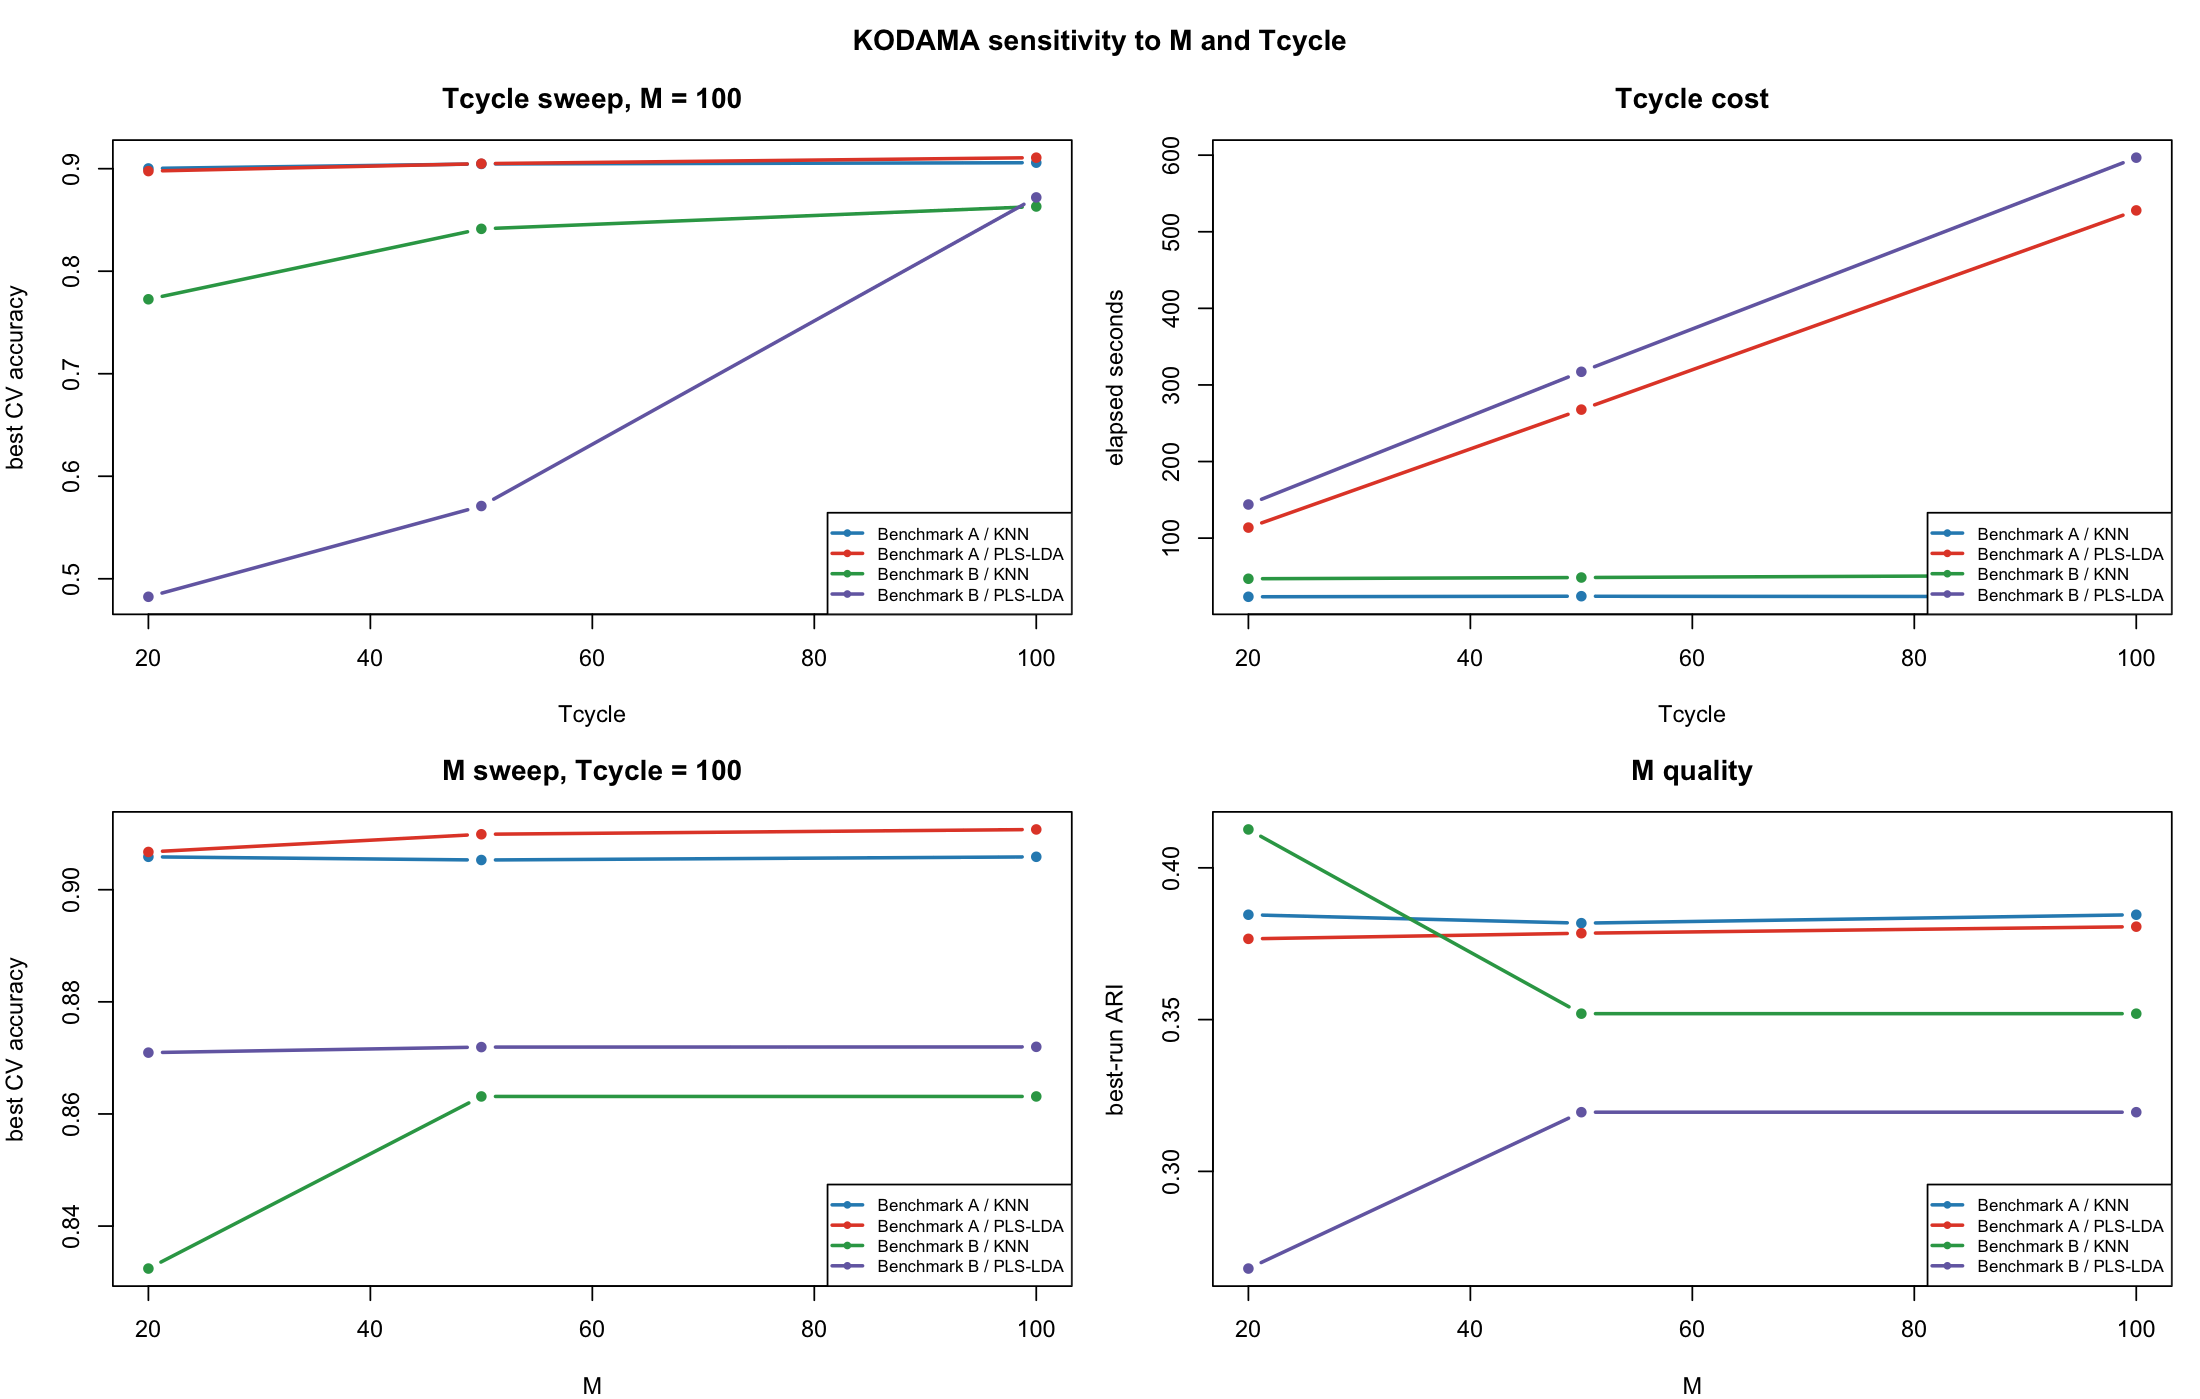
\includegraphics[width=\linewidth]{kodama_m_tcycle_sensitivity.png}
\caption{Sensitivity of KODAMA quality and runtime to Tcycle and M on named matrix-input datasets.}
\end{figure}

\begin{table}[h]
\caption{Convergence of agreement-graph edge weights. RMSE entries show M = 10 / 20 / 50 relative to M = 100.}
\small
\begin{tabular}{llll}
\toprule
Dataset & Classifier & RMSE to M100 & Correlation at M50 \\
\midrule
MetRef & KNN & 0.1377 / 0.0783 / 0.0407 & 0.9888 \\
MetRef & PLS-LDA & 0.0588 / 0.0453 / 0.0180 & 0.9988 \\
USPS & KNN & 0.1011 / 0.0617 / 0.0319 & 0.9955 \\
USPS & PLS-LDA & 0.1191 / 0.0803 / 0.0380 & 0.9926 \\
\bottomrule
\end{tabular}
\end{table}

\begin{figure}[h]
\centering
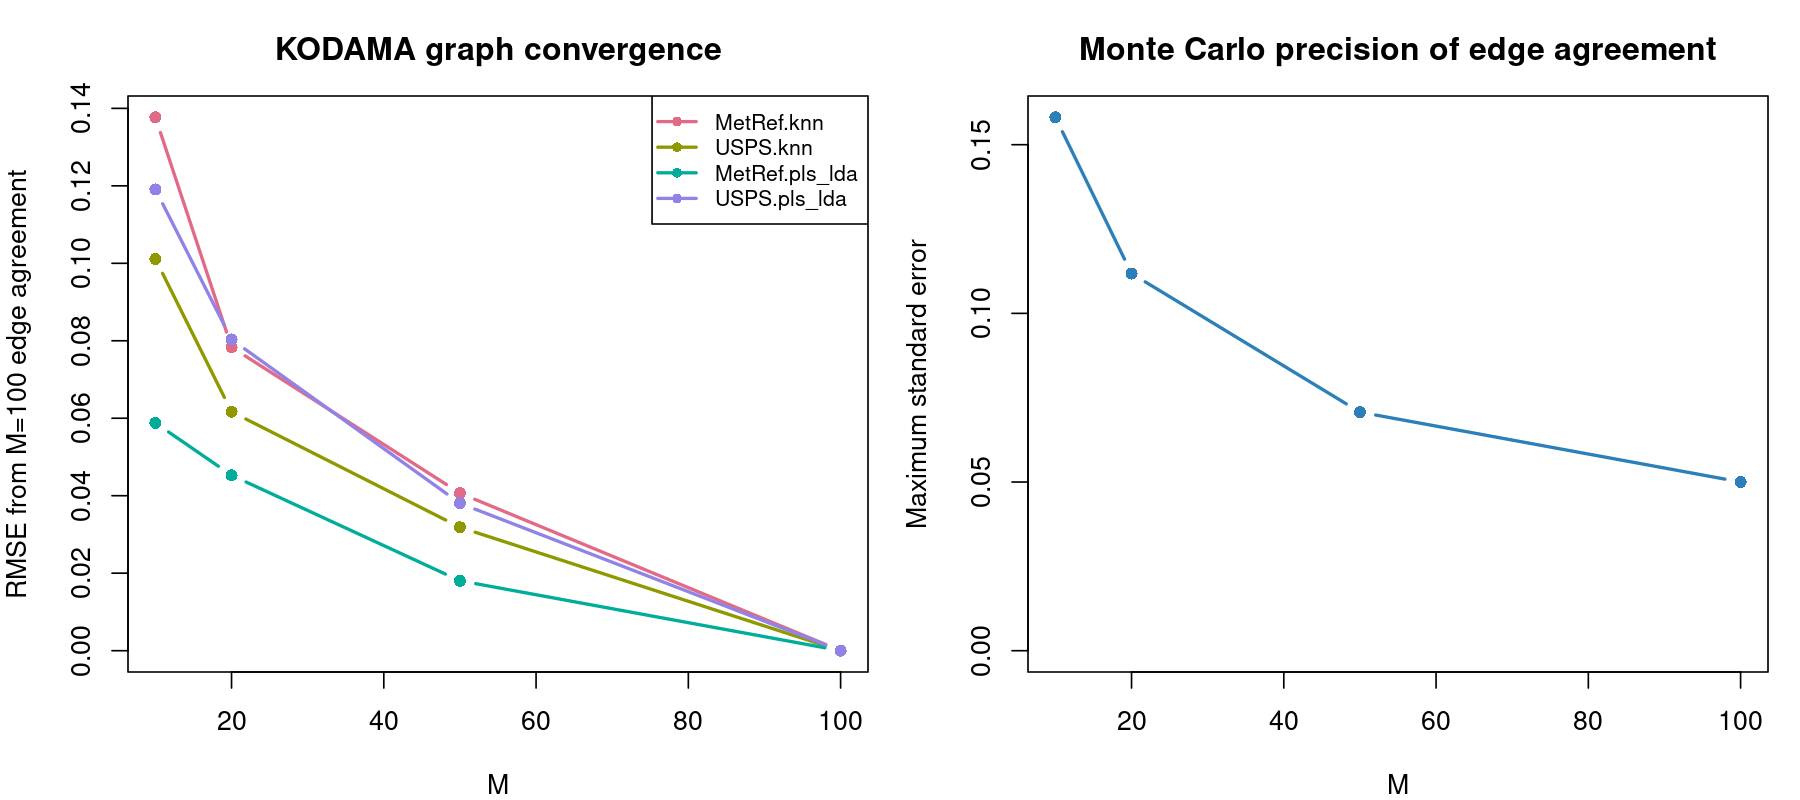
\includegraphics[width=\linewidth]{jmlr_pilot_20260716/ensemble_convergence.png}
\caption{Convergence of edge-agreement weights as independent KODAMA runs are added. RMSE is measured against M = 100; the right panel shows the Bernoulli worst-case Monte Carlo standard error.}
\end{figure}

\subsection{Implementation claims and archived evidence}
Source locations, tests, rejected alternatives, and backend measurements are archived in the repository's dated full-code audit, benchmark index, and checksum-bearing CSV files. The supplement reports the decisive aggregates rather than duplicating that machine-auditable matrix.

\begin{table}[h]
\caption{Release claims and required evidence.}
\small
\begin{tabularx}{\linewidth}{p{0.20\linewidth}X}
\toprule
Claim & Evidence contract \\
\midrule
Correctness & CTest passed on dependency-free CPU, Apple Metal, and CUDA builds; tests cover constrained folds, predictions, confusion matrices, requested component counts, and backend parity. \\
Numerics & Float32 MatrixView validation tests exercise CPU, CUDA, and Metal KNN/PLS-LDA paths with typed backend metadata; a fresh CUDA configure/build verifies that SIMPLS has no Armadillo or double-fallback dependency. \\
Performance & Kernel-level KNNCV/PLSLDACV timings are separated from core optimizer and KODAMA.matrix timings in the benchmark outputs. \\
Continuous integration & GitHub Actions commit a32f718 passed the CI, CPU-coverage, and API-documentation workflows, including Linux/macOS CPU, native Metal, and wrapper jobs. \\
Coverage and documentation & LLVM 22.1.1 CPU instrumentation measured 80.48\% line, 69.33\% branch, 77.50\% function, and 79.98\% region coverage. Dedicated graph-construction and clustering contract tests raised graph\_cluster.cpp to 94.65\% line and 73.94\% branch coverage. Cycles 19--22 added invalid-input, visualization-option, binary-UMAP compaction/replay, empty-resident-index, unavailable-backend, fixed-seed replay, monotone best-trace, guarded one-class, anti-collapse, shake-recovery, constant-predictor PLS-LDA fallback, and generic raw/graph matrix-orchestration contracts. Cycle 26 added resident-IVF null-view, non-positive-k, unavailable-backend, and move-ownership contracts. CUDA and Metal are excluded from that CPU number and retain hardware tests. Doxygen generation and GitHub Pages deployment passed, and the public API site is reachable at https://tkcaccia.github.io/kodama-cpp/. \\
Release & CMake install targets, wrapper build scripts, SPDX source headers, a pinned provenance matrix, retained third-party license texts, and a checksum-backed license audit are present. On 2026-08-06 the public main branches were core 0b8b8736e4ef688e0fccb4c86057ef455de88760 and R wrapper 709059237266c741898d720e650bf3e38e92e7ec. Neither is a release tag, and the uploaded HPC manifests contain git\_commit = NA; the final benchmark must therefore be rerun from a clean tagged archive rather than attributed retrospectively. \\
\bottomrule
\end{tabularx}
\end{table}

\section{Availability and reproducibility}
kodama-cpp is intended for release in the public tkcaccia/kodama-cpp GitHub repository. Original project code is licensed under MIT, while identified compatible third-party portions retain their upstream terms. In particular, the Metal backend is marked MIT AND Apache-2.0 because its fastEmbedR lineage retains the Faiss-mlx fused list-scan/top-k organization under Apache-2.0. The reviewed release architecture is a standalone C++17 core repository, a separate R wrapper repository, and Python binding source versioned with the core.

Reproducibility is supported through CMake builds, CPU, CUDA, and Metal tests, wrapper validation tests, benchmark scripts, and explicit recording of backend parameters. GitHub Actions builds and tests the CPU core on Linux and macOS, builds the native Metal core on macOS, and installs and tests both wrapper packages. A separate LLVM workflow measures CPU source coverage, while Doxygen publishes the typed API and a compact C++/R/Python walkthrough at https://tkcaccia.github.io/kodama-cpp/. The C++ core does not depend on R data readers; wrappers translate host-language objects into contiguous matrices before calling the library.

As of 6 August 2026, the public main branches identify abbreviated core commit 0b8b873 and R-wrapper commit 7090592. Neither repository yet has an immutable release tag, the Python wrapper is still distributed within the core source tree, and the uploaded HPC manifests record git\_commit as NA. The multi-dataset analysis is therefore reported as exploratory. A confirmatory release benchmark must be rerun from a clean tagged core and wrapper pair and record source checksums and the container digest.

A versioned provenance audit maps every shipped source-like file to an SPDX license identifier and records pinned KODAMA, fastPLS, fastEmbedR, faissR, FAISS, Faiss-mlx, and cuVS snapshots. Stefano Cacciatore confirmed that tkcaccia is his historical Git identity and separately authorized MIT distribution of the KODAMA and fastPLS-derived portions whose copyright he owns. The audit preserves publication coauthor credit, third-party notices, and full license texts, and is enforced by a release-time source-header and retained-license checksum test.

\subsection{Installation, wrappers, and licensing}
CMake configures the standalone core for CPU, native Apple Metal, or NVIDIA CUDA. Thin R and Python packages link to the installed core. Build and compatibility records are maintained in \path{README.md}, \path{docs/getting-started.md}, and \path{docs/r-api.md}. Licensing boundaries are defined by \path{PROVENANCE.md}, \path{THIRD_PARTY_NOTICES.md}, SPDX headers, retained license texts, and the automated audit.

\section{Limitations}
KODAMA performs $M(T+1)$ repeated CV evaluations and can remain expensive even when graph construction is fast. PLS-LDA is especially costly for large landmark sets or many predictors. Landmark selection and proposal control remain host-orchestrated; fully device-side evolution is not claimed.

The main engineering limitation is that KODAMA performs many cross-validation fits. This makes memory locality, buffer reuse, label compaction, and GPU scheduling as important as asymptotic complexity. The present release includes float32 buffers, fold reuse, label compaction, a resident full-data graph, persistent per-worker CUDA/Metal classifier workspaces, and native accelerator KNN and PLS-LDA kernels. Landmark selection and proposal control remain host orchestrated; a fully device-side evolutionary state machine is an engineering extension rather than a claim of the current manuscript.

The native CUDA neighbor-graph builder currently supports at most 256 retained neighbors per sample, whereas the CPU path supports larger rows. The implementation raises an error rather than silently truncating k. Benchmark protocols therefore record unsupported graph sizes as missing and never manufacture an accelerator row by changing a requested parameter.

The classic-versus-KODAMA archive is exploratory because earlier manifests lack a source commit. Its results demonstrate both favorable and adverse behavior and are excluded from release-level performance claims.

\section{Availability, wrappers, and provenance}
The standalone core is hosted at \url{https://github.com/tkcaccia/kodama-cpp}; the R wrapper is hosted at \url{https://github.com/tkcaccia/kodama-r}. Python binding source is versioned with the core. The project provides CMake install targets, API documentation, issue tracking, contribution guidance, benchmark drivers, and wrapper installation instructions.

Original project code is MIT licensed. Identified third-party-derived portions retain compatible upstream terms; the Metal list-scan/top-k lineage is marked MIT AND Apache-2.0. \path{PROVENANCE.md}, \path{THIRD_PARTY_NOTICES.md}, retained license files, source SPDX headers, and the automated license audit define the distribution boundary. Historical KODAMA, fastPLS, fastEmbedR, faissR, FAISS, Faiss-mlx, and cuVS revisions are recorded for attribution and audit; none is a runtime dependency of the standalone library.

Output:
  y_best: optimized labels for this run
  pred_best: CV predictions attached to y_best
  acc_best: raw CV accuracy of y_best

pred0 <- CrossValidate(F, X_L, y0, folds)
acc0 <- Accuracy(y0, pred0)
score0 <- ObjectiveScore(F, y0, acc0)
y_best <- y0; pred_best <- pred0; acc_best <- acc0; score_best <- score0
y_current <- y0; pred_current <- pred0; acc_current <- acc0; score_current <- score0

for t = 1,...,Tcycle do
  if evolutionary_search then
    y_base <- y_current; pred_base <- pred_current
  else
    y_base <- y_best; pred_base <- pred_best
  end if

  y_prop <- y_base
  qmax <- ProposalBudget(t, Tcycle, number_of_groups)
  q <- UniformInteger(1, qmax)
  selected_groups <- SampleWithoutReplacement(groups, q)

  for each group g in selected_groups do
    E <- {i in members(g): fixed[i] != 1}
    if E is empty then continue
    replacement <- SampleEmpirical(pred_base[E])
    y_prop[E] <- replacement
  end for

  y_prop <- ClassTransitionProposals(y_prop, pred_base, fixed)
  if F == PLS-LDA then
    y_prop <- PLSLDATransitionCoarsening(y_prop, pred_base, fixed)
  end if
  pred_prop <- CrossValidate(F, X_L, y_prop, folds)  # exactly one CV pass
  acc_prop <- Accuracy(y_prop, pred_prop)
  score_prop <- ObjectiveScore(F, y_prop, acc_prop)

  if score_prop > score_best then
    y_best <- y_prop; pred_best <- pred_prop
    acc_best <- acc_prop; score_best <- score_prop
  end if

  if evolutionary_search and
     Accept(score_prop, score_current, acc_current, t, Tcycle, rng) then
    y_current <- y_prop; pred_current <- pred_prop
    acc_current <- acc_prop; score_current <- score_prop
  end if

  if acc_prop == 1 and (!guarded_diversity or score_prop >= score_best) then break
end for

return y_best, pred_best, acc_best
\end{verbatim}
\end{scriptsize}

The compact ensemble pseudocode in Section 2.5 and the graph-input contract in Section 3.8 define KODAMA.matrix and KODAMA.matrix.graph without repeating the same steps here. Executable C++, R, and Python examples are maintained in the public API documentation.

\acks{The authors thank contributors to the KODAMA, fastPLS, and fastEmbedR software projects.}
\bibliography{kodama_cpp_refs}
\end{document}
